%% LyX 2.1.4 created this file.  For more info, see http://www.lyx.org/.
%% Do not edit unless you really know what you are doing.
\documentclass[11pt,czech,american]{book}
\usepackage[T1]{fontenc}
\usepackage[utf8]{inputenc}
\usepackage[a4paper]{geometry}
\geometry{verbose,tmargin=4cm,bmargin=3cm,lmargin=3cm,rmargin=2cm,headheight=0.8cm,headsep=1cm,footskip=0.5cm}
\pagestyle{headings}
\setcounter{secnumdepth}{3}
\usepackage{url}
\usepackage{amsmath}
\usepackage{amsthm}
\usepackage{amssymb}
\usepackage{graphicx}
\usepackage{setspace}
\usepackage[final]{pdfpages}
\usepackage{natbib}
\usepackage{mathrsfs}
\usepackage{algorithm}
\usepackage{algorithmicx}
\usepackage[noend]{algpseudocode}
\usepackage{caption}

\usepackage{array}
\usepackage{ragged2e}

\usepackage{lipsum}
\usepackage{psvectorian}

\DeclareMathOperator*{\argmax}{arg\,max}

\makeatletter
%%%%%%%%%%%%%%%%%%%%%%%%%%%%%% Textclass specific LaTeX commands.
\newenvironment{lyxlist}[1]
{\begin{list}{}
{\settowidth{\labelwidth}{#1}
 \setlength{\leftmargin}{\labelwidth}
 \addtolength{\leftmargin}{\labelsep}
 \renewcommand{\makelabel}[1]{##1\hfil}}}
{\end{list}}

%%%%%%%%%%%%%%%%%%%%%%%%%%%%%% User specified LaTeX commands.
%% Font setup: please leave the LyX font settings all set to 'default'
%% if you want to use any of these packages:

%% Use Times New Roman font for text and Belleek font for math
%% Please make sure that the 'esint' package is turned off in the
%% 'Math options' page.
\usepackage[varg]{txfonts}

%% Use Utopia text with Fourier-GUTenberg math
%\usepackage{fourier}

%% Bitstream Charter text with Math Design math
%\usepackage[charter]{mathdesign}

%%---------------------------------------------------------------------

%% Make the multiline figure/table captions indent so that the second
%% line "hangs" right below the first one.
%\usepackage[format=hang]{caption}

%% Indent even the first paragraph in each section
\usepackage{indentfirst}

%%---------------------------------------------------------------------

%% Disable page numbers in the TOC. LOF, LOT (TOC automatically
%% adds \thispagestyle{chapter} if not overriden
%\addtocontents{toc}{\protect\thispagestyle{empty}}
%\addtocontents{lof}{\protect\thispagestyle{empty}}
%\addtocontents{lot}{\protect\thispagestyle{empty}}

%% Shifts the top line of the TOC (not the title) 1cm upwards 
%% so that the whole TOC fits on 1 page. Additional page size
%% adjustment is performed at the point where the TOC
%% is inserted.
%\addtocontents{toc}{\protect\vspace{-1cm}}

%%---------------------------------------------------------------------

% completely avoid orphans (first lines of a new paragraph on the bottom of a page)
\clubpenalty=9500

% completely avoid widows (last lines of paragraph on a new page)
\widowpenalty=9500

% disable hyphenation of acronyms
\hyphenation{CDFA HARDI HiPPIES IKEM InterTrack MEGIDDO MIMD MPFA DICOM ASCLEPIOS MedInria}

%%---------------------------------------------------------------------

%% Print out all vectors in bold type instead of printing an arrow above them
\renewcommand{\vec}[1]{\boldsymbol{#1}}

% Replace standard \cite by the parenthetical variant \citep
%\renewcommand{\cite}{\citep}

\makeatother

\usepackage{babel}

\newcommand{\ornamentleft}{%
	\psvectorian[width=2em]{2}%
}
\newcommand{\ornamentright}{%
	\psvectorian[width=2em,mirror]{2}%
}

\newcommand{\ornamentheader}[1]{%
	\begin{center}
		\ornamentleft
		\quad{\large\emph{#1}}\quad % style as desired
		\ornamentright
	\end{center}%
}

\newlength{\rlength}\setlength{\rlength}{16cm}
\newcommand{\ruletext}[2][\rlength]{%
	\noindent%
	\parbox{#1}{%
		\noindent\dotfill\raisebox{-.3\ht\strutbox}{#2}\dotfill\par}%
}





\begin{document}
\def\documentdate{July 7, 2017}

\newtheorem{definition}{Definition}[chapter]
\newtheorem{note}{Note}[chapter]
\newtheorem{example}{Example} 
\newtheorem{assumption}{Assumption} 

\newtheorem{theorem}{Theorem}
\newtheorem*{remark}{Remark}

\captionsetup[figure]{labelfont={bf},labelformat={default},labelsep=period,name={Fig.}}

\def\documentdate{\today}

\pagestyle{empty}
{\centering

\noindent %
\begin{minipage}[c]{3cm}%
\noindent \begin{center}

\includegraphics[width=3cm,height=3cm,keepaspectratio]{Images/TITLE/cvut}
\par\end{center}%
\end{minipage}%
\begin{minipage}[c]{0.6\linewidth}%
\begin{center}
\textsc{\large{}Czech Technical University in Prague}{\large{}}\\
{\large{}Faculty of Nuclear Sciences and Physical Engineering}
\par\end{center}%
\end{minipage}%
\begin{minipage}[c]{3cm}%
\noindent \begin{center}

\includegraphics[width=3cm,height=3cm,keepaspectratio]{Images/TITLE/fjfi}
\par\end{center}%
\end{minipage}

\vspace{3cm}


\textbf{\huge{}Real Options Valuation: A Dynamic Programming Approach}{\huge \par}

\vspace{1cm}


\selectlanguage{czech}%
\textbf{\huge{}Oceňování Projektů Metodou Reálných Opcí z Pohledu Dynamického Progamování}{\huge \par}

\selectlanguage{american}%
\vspace{2cm}


{\large{}Master's Thesis}{\large \par}

}

\vfill{}

\begin{lyxlist}{MMMMMMMMM}
\begin{singlespace}
\item [{Author:}] \textbf{Filip Rolenec}
\item [{Supervisor:}] \textbf{Ing. Rudolf Kulhavý, DrSc.}
\end{singlespace}

\item [{Language~advisor:}] \textbf{Ing. Rudolf Kulhavý, DrSc.} 
\begin{singlespace}
\item [{Academic~year:}] 2020/2021\end{singlespace}

\end{lyxlist}
\newpage{}

~\newpage{}

~

\vfill{}


\begin{center}
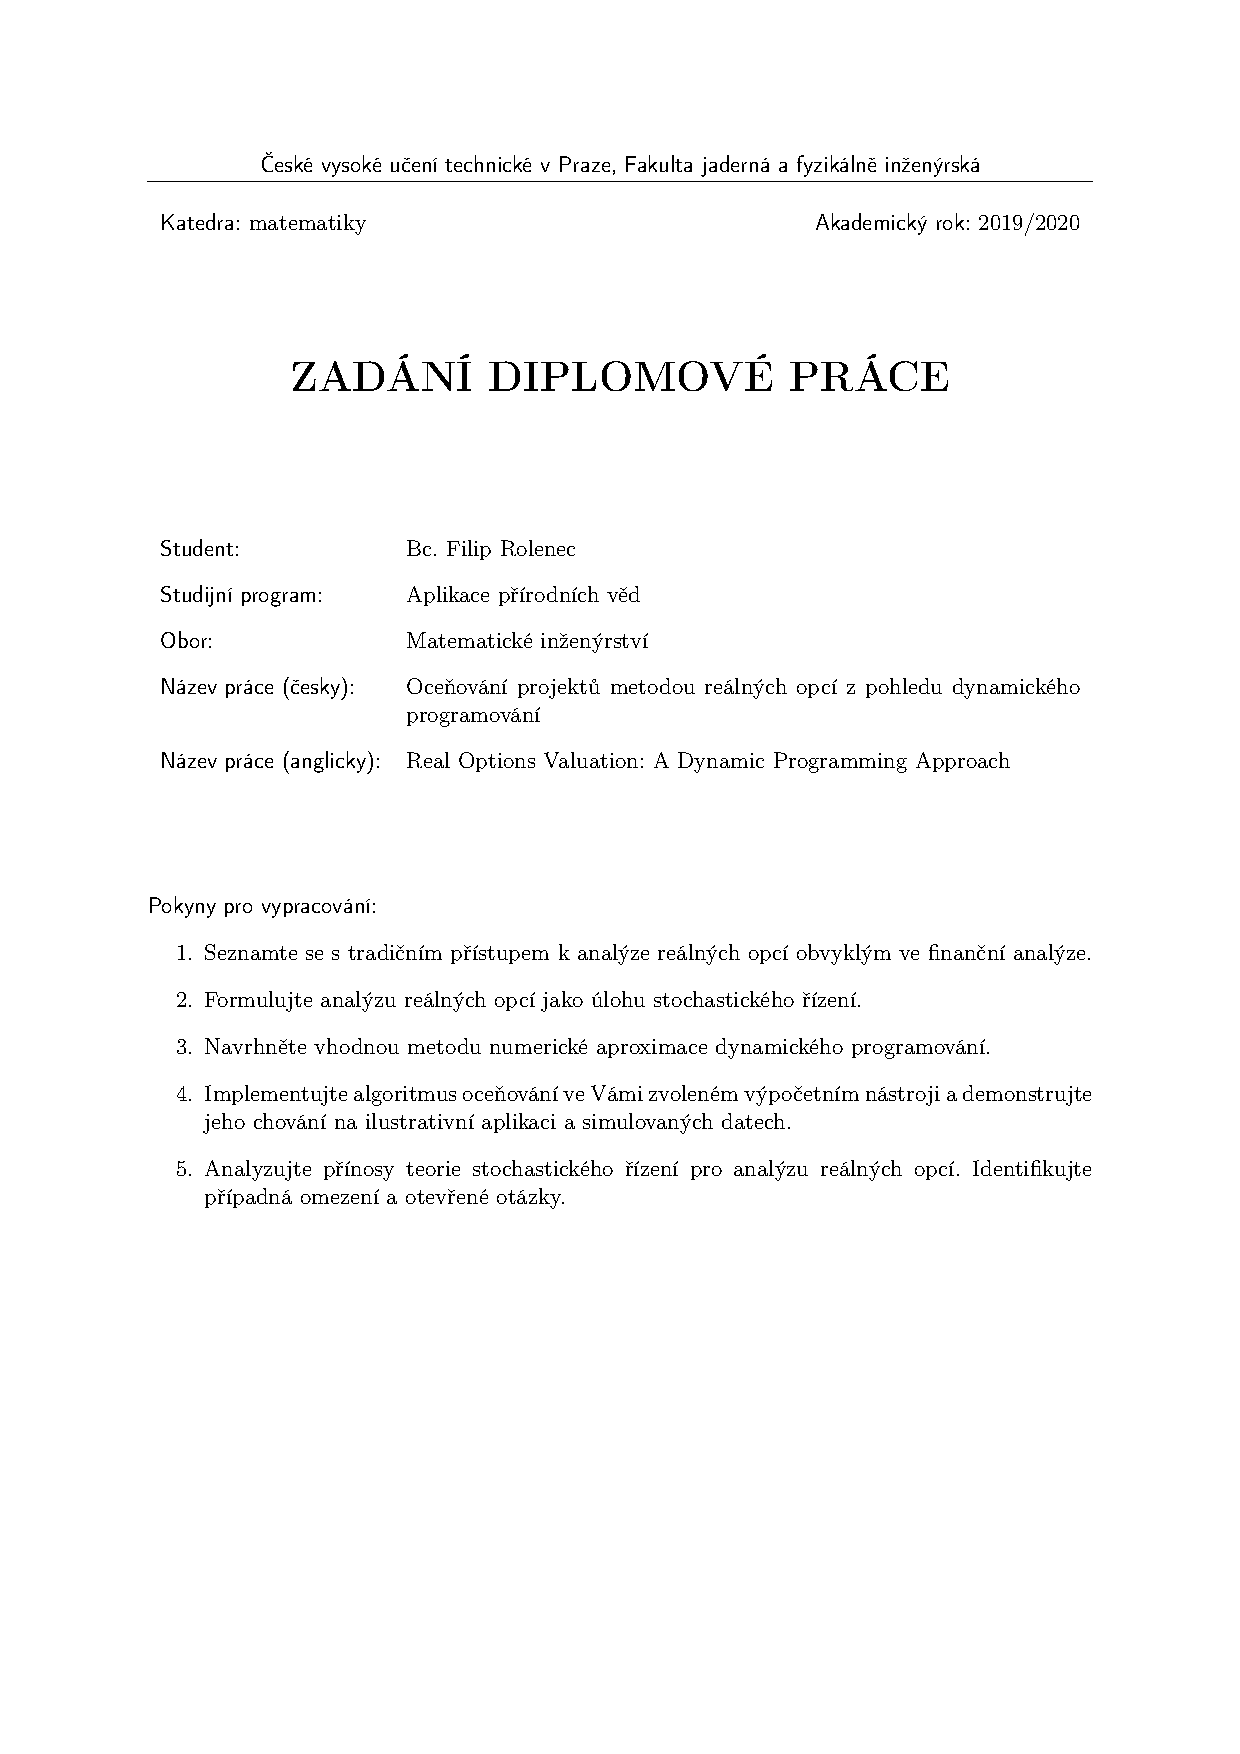
\includepdf[pages={1}]{Images/zadaniMT.pdf}


\par\end{center}

\vfill{}


~\newpage{}

~

\vfill{}


\begin{center}
\includepdf[pages={2}]{Images/zadaniMT.pdf}
\par\end{center}

\vfill{}


~\newpage{}

\noindent \emph{\Large{}Acknowledgment:}{\Large \par}

\noindent I would like to thank my supervisor Ing. Rudolf Kulhavý, DrSc. for his professional guidance and all the advice given while creating this thesis. 

\vfill

\noindent \emph{\Large{}Author's declaration:}{\Large \par}

\noindent I declare that this Master's thesis is entirely
my own work and I have listed all the used sources in the bibliography.

\bigskip{}


\noindent Prague, \documentdate\hfill{}Bc. Filip Rolenec

\vspace{2cm}


\newpage{}

~\newpage{}

\selectlanguage{czech}%
\begin{onehalfspace}
\noindent \emph{Název práce:}

\noindent \textbf{Oceňování Projektů Metodou Reálných Opcí z Pohledu Dynamického Progamování}
\end{onehalfspace}

\bigskip{}


\noindent \emph{Autor:} Bc. Filip Rolenec

\bigskip{}


\noindent \emph{Obor:} Matematické inženýrství 


\bigskip{}


\noindent \emph{Druh práce:} Diplomová práce

\bigskip{}


\noindent \emph{Vedoucí práce:} Ing. Rudolf Kulhavý, DrSc.


\bigskip{}


\noindent \emph{Abstrakt:} Teorie reálných opcí (ROA) je pokročilá valuační technika projektů, která respektuje hodnotu možných budoucích změn (tzv. \textit{reálných opcí}). 

Domníváme se, že v současné ROA neexistuje obecný algoritmus pro valuaci komplexních projektů, kterými myslíme projekty s více náhodnými veličinami a větším množstvím projektových alternací různého typu. 

Tato diplomová práce se inspiruje problémem oceňování ve smyslu ROA a snaží se ho interpretovat jako problém dynamického rozhodování za neurčitosti z oblasti statistické teorie rozhodování (SDT). V práci představujeme obecný valuační algoritmus, který staví na poznatcích ze SDT, pokrývá problémy řešené současnou ROA a navíc respektuje vliv ekonomických konceptů jako je časová hodnota peněz a averze vůči riziku investorů. 

Použití jmenovaného algoritmu je představeno na problému ocenění plynové elektrárny, kde problém nespočetného stavového prostoru řešíme pomocí techniky přibližného dynamického programování nazývané aproximace hodnotové funkce. Hodnotové funkce modelujeme jako součet po částech lineárních funkcí, tak aby odrážely opční strukturu projektových odměn. 
 
\bigskip{}


\noindent \emph{Klíčová slova:}   Analýza reálných opcí, Blackův-Scholesův model, Čistá současná hodnota, Dynamické programování, Energetika, Oceňování projektů, Statistická rozhodovací teorie



\selectlanguage{american}%
\vfill{}
~

\begin{onehalfspace}
\noindent \emph{Title:}

\noindent \textbf{Real Options Valuation: A Dynamic Programming Approach}
\end{onehalfspace}

\bigskip{}


\noindent \emph{Author:} Bc. Filip Rolenec

\bigskip{}


\noindent \emph{Abstract:} The theory of real option analysis (ROA) is considered as an advanced project valuation technique, which respects the value of future project alternations (\textit{real options}). 

 To our best knowledge, the current state of ROA does not offer a unified valuation algorithm that would be able to cover valuations of more complex projects, such as those with multiple random variables or different types and a larger number of possible actions. 
	
This thesis takes the problem of ROA and tries to interpret it as a problem of decision making under uncertainty from the statistical decision theory (SDT).
We present a general valuation algorithm that builds on the knowledge of SDT, covers the solutions proposed by ROA, and preserves the business-specific concepts as time value of money and risk-aversion of investors.  

This algorithm's usage is demonstrated on a problem of gas power plant§s valuation, where the problem of uncountable state space is solved via the approximate dynamic programming technique of value function approximation, where we use piecewise linear models to cover the option-like structure. 
	
	
\bigskip{}


\noindent \emph{Keywords:} Black-Scholes model, Dynamic programming, Net present value, Power industry, Project valuation,  Real option analysis, Statistical decision theory

\newpage{}

~\newpage{}

\pagestyle{plain}

\tableofcontents{}

\newpage{}

\chapter{Introduction}
Investing is a problem of optimal allocation of resources (mostly money) between investor's alternative choices. Two main groups of investments can be recognized as first, the investment in the financial (or commodity) market, and second, the direct investment in business ventures. The first type of investment can be approached by a deeper mathematical analysis as it consist of a relatively limited number of different products traded in large quantities, producing huge analyzable datasets. Such structured datasets do not exist for the second type of investment and thus it cannot be approached in the same sense.  

In this thesis, we will focus on investments in projects (new businesses or alternations of old ones), where the problem of resource allocation between various opportunities is being solved with the metric of project valuation. From the various project valuation techniques, we have chosen the theory of real options (ROA) as an inspiration for creating a valuation model based on the ideas of statistical decision theory (SDT).

First, we describe the historical background of the ROA valuation. Next, we focus on the reasons why we investigate the idea of SDT interpretation of ROA. In the remainder of this chapter, we present the outline of this thesis. 

\section{Historical Background - Real Options}

The foundations of financial derivatives\footnote{Derivatives are financial arrangements between two parties whose payments are based on, or ``derived`` from, the performance of some agreed-upon benchmark. They can be issued on currencies, commodities, government or corporate debt, home mortgages, stocks, interest rates, or any combination \cite{BodKan:04}. } date back to the origins of commerce in Mesopotamia in the fourth millennium BC \cite{Web:09}. The derivative market consisted mainly of forward contracts\footnote{A forward contract is a contract to purchase an asset at a fixed price on a particular date in the future \cite{BerDeM:09}.} and it was introduced to the European continent through Spain in Roman times. After the expulsion of derivative trading in Spain the center of this type of commerce for Europe were the Low Lands, where at the end of the 17th century, the first ideas about options\footnote{A financial option is the \textit{ability} to buy (call option) or sell (put option) a defined volume of an asset for a specified amount of money at some future time instant \cite{BerDeM:09}.}  and option trading were published by La Vega \cite{Veg:88}. 

The first attempts of a mathematical option pricing come from Bachelier (1900) \cite{Bac:00} and Bronzin  (1908) \cite{Bro:08}. Based on their work, the boom of option pricing methods in the 1970's culminated in Nobel-prize-awarded Black-Scholes model (BSM) \cite{BlaSch:73}, which is today's standard in the financial option pricing theory \cite{YalHak:12}. 

The publicity and wide adoption of the BSM most likely inspired an expert on capital budgeting, Stewart Myers, to introduce the term ``real options`` \cite{Mye:77}, one of two main pillars of this thesis. Myers builds on the idea that real options - the ability to alter the project in the future - are able to bring significantly larger value in comparison to the same project without them. Myers' approach to the real options is mostly philosophical in a sense that he stresses out the importance of thinking about the additional value real options can bring. At the same time, he does not present any computational tool for the said value. 

The idea of real option analysis (ROA) as a valuation tool for projects was further developed by several influential authors in the following decades, for example Guthrie \cite{Gut:09}, Pindyck \cite{DixPin:12} or Kulatilaka \cite{AmrKul:98}. 

The valuation of project's free cash flows with ROA is in corporate finance understood as very advanced, and its adoption in practice is slow \cite{Amp:17}. It is argued that this slow adoption is caused mainly by misunderstanding the more difficult mathematical concept of ROA \cite{SicGam:10} and the low adoption rate of a competition: ``Why should our company use a new tool that no one else is using?`` \cite{CopAnt:01}. 

\section{Research Motivation}
Through the author's studies at FNSPE CTU, he has specialized in the theory of dynamic decision-making under uncertainty. In his final years at the university he also became curious about the world of corporate finance, since he was working for a venture capital investor Presto Ventures. This combination of his professional interests is pleasantly reflected in the assignment of this thesis - the interpretation of ROA in terms of SDT. 

Through the study of the ROA state of the art, we have found out that the term \textit{real options} is not clearly defined. As will be illustrated in-depth in section \ref{sec:ROA} we identify three classes of ROA authors based on the level of analogy to the BSM model. 

In this thesis, we focus on the class of ROA authors, which utilize only the non-arbitrage principle to determine the probabilities of used models. We build mostly on the state-of-the-art textbook from Guthrie \cite{Gut:09} and the analysis of the  potential real option representation via SDT from Vollert \cite{Vol:03}.

The goal of this thesis is to take the project valuation problem structure as is understood in ROA and look at it from the SDT perspective. One of the challenges of this task is to implement the business-specific concepts about investors' behavior and the way they perceive value.  Two main addressed concepts are the time value of money and the risk aversion of investors. 

The goal of this thesis is to provide an SDT-based valuation algorithm for projects, whose value is understood as a maximal possible present cash equivalent (PCE)\footnote{A proposed valuation metric that incorporates the capital management of a project.} of the uncertain future cash flows. This valuation algorithm covers the classes of problems now solved by ROA and allows for new ones. 

The new SDT based valuation algorithm enables: 
\begin{itemize}
	\item seamless integration of multiple uncertainty sources;
	\item integration of theoretically any probability distribution as a model of uncertain variables;
	\item usage of a high number of possible actions (options), regardless of their nature; 
	\item utilization of approximate dynamic programming tools for high-dimensional problems;
	\item preservation of the business-specific concepts as time value of money and the risk aversion of investors. 
\end{itemize}

To illustrate the usage of the new SDT-based algorithm a valuation of a project from a selected class is performed. This class is denoted as \textit{simple flow businesses} and is defined as the type of businesses that can, for the purpose of their valuation, be described by a straightforward transformation of inputs to outputs. It covers all projects whose cycle time is equal to zero, and the input-output transformation rate is constant. This class is a generalization motivated by an example of a gas power plant valuation presented by Guthrie in \cite{Gut:09}. 

\section{Outline of the Thesis}

The thesis is structured into 7 chapters, introduction being the first.

Chapter 2 defines the mathematical notation and presents the mathematical concepts used through the thesis. Useful probability concepts are reminded at the beginning, while the rest of the chapter is reserved for the SDT. 

Chapter 3 introduces the second pillar of this thesis, which is the economic concept of a project valuation. The chapter begins with a description of a classic valuation technique called the net present value NPV, which is, for the purpose of this thesis, upgraded to a new concept of present cash equivalent (PCE). The remainder of the chapter is left for the discussion about financial and real options. 

Chapter 4 represents the core of this thesis. First, we define what will be understood as a problem of ROA project valuation. We state the key features that define a project, and we limit these features accordingly. Then we focus on the interpretation of the problem by a general SDT framework. We illustrate the identification of ROA project features in SDT. The remainder of the fourth chapter is reserved for resolving the economic nuances that need to be accounted for in the SDT framework in order to make the valuation procedure consistent with the economic reality of investors' behavior. 

Chapter 5 illustrates the new valuation algorithm from chapter 4 on a valuation example of a simple flow business. A valuation of a gas power plant is chosen as the representative of this class. The first half of the chapter focuses on the value sensitivity with regard to the volume of available managerial actions in the project. The second half presents a value comparison  of project alternations in different price variances, and it is aimed to demonstrate the increase in value of a more uncertain environment. 

Chapter 6 discusses the new findings, both theoretical and observed from the performed experiments. 

Chapter 7 summarizes the thesis - reminds the motivation, underlines the main message, and lists all contributions of this thesis. Furthermore, it outlines many possible future research paths in this field as it is, to our best knowledge, the first available publication on this topic. 


%\addcontentsline{toc}{chapter}{Introduction}

%\addcontentsline{toc}{chapter}{Preliminaries}

\pagestyle{headings}



\chapter{Preliminaries}
To properly understand a mathematical text, it is essential to first define the used symbolism and notions. The used mathematical notation comes from influential authors in their respective fields of study: 

\begin{itemize}
	\item statistical decision theory - Bacci and Chiando \cite{BacChi:19} and Puterman \cite{Put:05};
	\item probability theory - Jaynes \cite{Jay:03};
	\item approximate dynamic programming - Powel \cite{Pow:11}.
\end{itemize}

 The pure mathematical symbolism comes from the author's studying experience at FNSPE CTU demonstrated also in his previous publications \cite{Rol:18} and \cite{Rol:19}. 


\section{Probability Theory}
In the whole thesis, bold capital letters, such as $\mathbf{X}$, represent a set of all elements $x \in \mathbf{X}$ as in \cite{Rol:18}. The cardinality of a set $\mathbf{X}$ is denoted with two vertical lines as $|\mathbf{X}|$. 

Random variables, understood in the sense of the standard Kolmogorov's probability theory \cite{Kol:60}, are denoted with a tilde above the variable, e.g., $\tilde{x}$. Values of random variables are denoted by the same letters as the random variable without the tilde, e.g., $x$. 

\begin{definition}(Probability)
	Let $\tilde{x}$ be a discrete random variable. Then $P(x)$ denotes a value of the probability mass function (p.m.f.)  for the realization $\tilde{x}=x$. Similarly, if $\tilde{x}$ is a continuous random variable, then $p(x)$ denotes a probability density function (p.d.f.) at $x$. 
\end{definition}

Next, we define the well-known concept of conditional probability \cite{Jay:03}. 
\begin{definition}(Conditional probability) 
	Let symbol $P(x|y)$ represent the conditional probability of a discrete random variable. Then the $P(x|y)$ is defined as:
	\begin{equation}
	P(x|y)=\frac{P(x,y)}{P(y)},
	\end{equation} where $P(x,y)$ is a joint p.m.f. of $\tilde{x}$ and $\tilde{y}$. 
\end{definition}

A similar concept is also used for the continuous random variables with the name of conditional probability density \cite{Jay:03}. 

\begin{definition}(Conditional probability density)
	Let symbol $p(x|y)$ represent the conditional probability density of a continuous random variable. Then the $p(x|y)$ is defined as:
	\begin{equation}\label{eq:condP}
	p(x|y)=\frac{p(x,y)}{p(y)},
	\end{equation} where $p(x,y)$ is a joint p.d.f. of $\tilde{x}$ and $\tilde{y}$. 
\end{definition} 

\begin{definition}(Expected value)
	Expected value of a discrete random variable $\tilde{x}$ is defined as: 
	\begin{equation}
		E[\tilde{x}]=\sum_{\mathbf{X}} P(x) x. 
	\end{equation}
	Similarly, for the continuous random variable $\tilde{y}$ the expected value is defined as: 
	\begin{equation}
	E[\tilde{y}]=\int_{\mathbf{Y}} p(y) y \ dy. 
	\end{equation}
\end{definition}


\subsection{Probability distributions}
Through this thesis, the following distributions will be referenced, either as an expected model of some random variable or in a broader discussion \cite{Bli:19}. 

\paragraph{Bernoulli distribution}
The Bernoulli distribution $Be(p)$ models the probability of success (1) or failure (0) with $p \in [0,1]$ by the p.m.f.: 

\begin{equation}
P(\tilde{x} = x, p) =
\left\{
\begin{array}{ll}
p  & x=1\\
1-p & x=0.
\end{array}
\right.
\end{equation}
This distribution is widely used in ROA, usually for the modeling of the up (1) and down (0) movement of asset or commodity prices. 


\paragraph{Binomial distribution}
Binomial distribution $Bi(n,p)$ represents the number of successes of $n$ independent random variables distributed by $Be(p)$ with p.m.f.:

\begin{equation}
	P(\tilde{x}=k, n, p)=\binom{n}{k} \cdot p^k(1-p)^{n-k}, \ k \in \{0,1,2, \dots ,n\}. 
\end{equation}

This distribution is used in a popular ROA modeling tool - \textit{the binomial model} \cite{Gut:09}. The idea is that a random variable (price, quantity, \dots) evolves as a realization of consequential up or down movements distributed by $Be(p_u)$, where $p_u$ is the probability of the up movement. Each move then updates the variable's value by multiplying it by a given coefficient $U$ or $D$. To ensure that the number of possible values rises linearly and not exponentially with the number of time epochs, the model limits the parameters as $D=1/U$.

Based on the number of up movements $n_u$ (as a realization of $Bi(n, p_u)$) until the $n$-th time epoch, and the initial value $v_{init}$, the realization of the modeled variable can be expressed as: 

\begin{equation}
v = v_{init} \cdot U^{2n_u-n}.
\end{equation}


\paragraph{Poisson distribution}
Poisson distribution $Po(\lambda)$ is a popular discrete distribution used in modeling of the number of successes in a given time-interval, so-called ``arrivals`` \cite{Bli:19}. This distribution is used for modeling of the number of incoming emails or the number of earthquakes in a given area in one year. 

Its p.m.f. given parameter $\lambda$ is: 
\begin{equation}
	P(\tilde{x}=x, \lambda)= \frac{\lambda^xe^{-\lambda}}{x!}, \  x\in \{0,1,2,\dots\}.
\end{equation}

Also, it is worth noting that a Poisson distribution $Po(\lambda)$ with $\lambda = np$ is the limit distribution of a $Bi(n, p)$ for $n \to \infty$, if the product $\lambda = n p$, which is the expected value of the number of arrivals, remains constant.


\paragraph{Log-normal distribution}
Another useful distribution for this thesis is the log-normal distribution $LogN(\mu, \sigma)$. It represents a continuous random variable, a logarithm of which is distributed normally. 

The p.d.f. of such variable is:
\begin{equation}
	p(x)=\frac{1}{x\sigma\sqrt{2\pi}} \exp\left(\-\frac{(ln(x)-\mu)^2}{2\sigma^2}\right).
\end{equation}

This distribution is again used mostly for modeling of asset or commodity prices, arguably for two main reasons. The first is that its realizations are positive, and the second being that variance reflects not only the parameter $\sigma$ but also $\mu$, where $\mu$ usually represents the previous price. 


\section{Statistical Decision Theory} 
The first pillar upon which this thesis stands is the statistical decision theory (SDT). An area of applied mathematics that formalizes and studies optimal decision making of agents. As decision making under uncertainty in its broadest sense encapsulates the majority of human behavior, the class of problems it is able to solve (at least theoretically) is quite large. 

The SDT's primary focus is to determine the optimal strategy (a sequence of decisions) to act upon, generally in a dynamic and uncertain environment. The optimality of a given strategy is measured by some reward metric, in the simplest case by a pure monetary gain. This metric is, however, not sufficient for many applications, so a general metric of agent's reward via utility (described in section \ref{sec:utility}) is used. 



\subsection{Markov decision process}
In this thesis, we will be modeling the decision-making problems using the standard framework of the Markov decision process (MDP) \cite{Put:05}. 
\begin{definition}(Markov decision process)
	
	Markov decision process is defined by its five building blocks: 
	\begin{itemize}
		\item The set of time epochs - $\mathbf{T}$;
		\item The set of states in those epochs - $\mathbf{S_t}$, $t \in \mathbf{T}$;
		\item The set of actions in those states - $\mathbf{A_{s_t}}$, $s_t \in \mathbf{S_t}$, $t \in \mathbf{T}$;
		\item The reward function of transition from one state to another - $r(s_t, a_{t-1},s_{t-1})$, where $s_t, \in \mathbf{S_t}$, $s_{t-1}, \in \mathbf{S_{t-1}}$,  and $a_{t-1} \in \mathbf{A_{s_{t-1}}}$;
		\item Transition probabilities governing the transition from one state to another $p(s_t|a_{t-1},s_{t-1})$, where $s_t, \in \mathbf{S_t}$, $s_{t-1}, \in \mathbf{S_{t-1}}$,  and $a_{t-1} \in \mathbf{A_{s_{t-1}}}$.
	\end{itemize}
\end{definition}

\begin{remark}
	The set of time epochs, states and actions is usually known, defined by the structure of the decision making problem that is being solved. Reward and transition functions tend to be unknown, and they need to be estimated. 
\end{remark}

\begin{remark}
	For a further simplification of the text, we define $\mathbf{S} = \bigcup\limits_{t \in \mathbf{T}} \mathbf{S_t}$ and $\mathbf{A} = \bigcup\limits_{s \in \mathbf{S}} \mathbf{A_{s}}$.
\end{remark}


Usually, the biggest task in SDT is to correctly approach the uncertainty about transition probabilities between different states of a decision making problem. There are two approaches to parameter estimation in statistics, a classical approach, and a Bayesian approach. Since the Bayesian approach seems to fit the decision-making format better, allowing for the notion of prior probabilities, incorporating expert knowledge, and the possibility for smooth updating on newly observed data - it is a preferable choice. 

In this thesis, however, we will not go into the detail of the transition probability function's modeling, and we will assume it to be known. 

\vspace{1em}
As outlined above, the goal of SDT is to find the optimal strategy - sequence of actions. The optimality of such strategy is defined as it having the maximal expected cumulative reward among all eligible strategies $\mathbf{\Pi}$: 

\begin{equation}
	\pi^*=\argmax_{\pi \in \mathbf{\Pi}} E\left[\sum_{t\in \mathbf{T}} r(s_t,a_{t-1},s_{t-1})\Bigg|\pi\right].
\end{equation}

\begin{remark}
	This definition of the optimal strategy is used mainly for finite MDP's or MDP's with exponential discounting of future rewards. Alternative definitions of optimality, for example, maximal average reward per period, exist.
\end{remark}

 Due to the nature of project valuation, where projects are considered to be finite or their cash flow exponentially discounted, this thesis will focus on a metric based on the presented notion of expected cumulative reward. 

\subsection{Dynamic programming}\label{Sec:DP}
Finding the optimal policy by computing the expected reward for all policies $\pi \in \mathbf{\Pi}$ is due to the cardinality of $\mathbf{\Pi}$: 
\begin{equation}
|\mathbf{\Pi}|= \prod_{t\in\mathbf{T}} \prod_{s_t \in \mathbf{S_t}} |\mathbf{A_{s_t}}| 
\end{equation}  
a very demanding task, even for low-dimensional MDP's. 

To cope with such computational complexity clever algorithms were developed, most notably the dynamic programming (DP) approach and the reinforcement learning approach. In this thesis we will focus on the first one, which is based on the idea of backward induction.

 The core of dynamic programming is to define the so-called value function $v(s)$ on each of the possible states $s \in \mathbf{S}$. Each of the values is computed via the Bellman equation: 
\begin{equation}\label{eq:Bellman}
v(s_{t-1}) = \max_{a_{t-1} \in \mathbf{A_{s_{t-1}}}}\sum_{s_t \in \mathbf{S_t}} P(s_t|a_{t-1}, s_{t-1}) [r(s_t, a_{t-1}, s_{t-1})+v(s_t)].
\end{equation}

The value function represents the expected cumulative reward from a given state onward. The idea of computing this value through the backward induction is based on the truth that a sequence of actions is optimal if and only if its last action is optimal.  Optimal strategy comes together with the value function seemingly as a byproduct, where in each state, the optimal action is the argument maxima of the expression in equation \ref{eq:Bellman}. 

This approach significantly reduces the computational complexity to
\begin{equation}
	\sum_{t \in \mathbf{T}} \sum_{s_t \in \mathbf{S_t}} |\mathbf{A_{s_t}}|
\end{equation}
expected value computations. 

\begin{remark}
	For a constant number of states in each time epoch $|\mathbf{S_t}|$  and a constant number of actions in each state $|\mathbf{A_{s_t}}|$, this reduction is from $|\mathbf{A_{s_t}}|^{|\mathbf{S_t}|^{|\mathbf{T}|}}$  to $|\mathbf{A_{s_t}}|\cdot |\mathbf{S_t}|\cdot|\mathbf{T}|$.
\end{remark}

The reduction of computational complexity with the DP algorithm is significant. However, for the majority of real-world applications it is not sufficient. In reality, due to the structure of decision-making problems and their formulation, the cardinality of state space can explode even for fairly simple problems. 

The problem of remaining computational complexity of DP algorithm is in literature addressed as ``three curses of dimensionality`` by Powel \cite{Pow:11}, who, among others, proposes solutions under the label of approximate dynamic programming (ADP). 


\subsection{Approximate dynamic programming}
The computational complexity of dynamic programming for middle and high-dimensional MDP's is so demanding that its results cannot be obtained in a reasonable amount of time. 

To cope with this problem, a relevant topic to look at is the section of SDT called approximate dynamic programming (ADP). The ADP label can be understood as a unifying name for a number of algorithms trying to obtain quasi-optimal strategies for decision-making problems with reasonable demands for computational power\footnote{For details, please see Powell \cite{Pow:11}.}. 

ADP algorithms can be divided into two main classes, policy and value iteration algorithms. In this thesis, we will be focusing on the value iteration class since we believe that due to the structure of project valuation problems (rather large $|\mathbf{S}$| and rather small $|\mathbf{A}|$), it is a better fit.

The idea of value iteration is to have some initial heuristic value function approximation, which is being updated based on samples of possible paths. 

In this section of the thesis, we present the most general form of the value function approximation model, which aims to describe the general shape of the value function by a small number of parameters\footnote{A value function is in classical DP similar to a look-up table. There is no simple functional relationship between states and the values of value functions.}. We will model the value function in each time epoch $v_t$ as a function of the state $s$ itself and a parametric function $f$ as: 

\begin{equation}\label{eq:genADP}
v_t(s) = f(s, \theta_{i,t} ),  \quad \theta_{i,t} \in \mathbf{\Theta_t},
\end{equation} 
where the cardinality $|\mathbf{\Theta_t}|$ is finite and preferably small. 

\begin{remark}
	To clarify the general formula represented by the equation \ref{eq:genADP}, we present an example, where the parametric function $f$ is a linear combination of some basis functions $\phi_{i}$: 
	\begin{equation}
	v_t(s) = \sum_{i} \theta_{i,t} \cdot \phi_{i}(s),
	\end{equation} 
	where each of the basis functions $\phi_{i}$ represents some heuristically important feature of each state $s \in \mathbf{S}$.  A project valuation example of such basis function might be a difference between state elements representing prices of inputs and outputs or indicator function of a state element representing the running production.
\end{remark}

\begin{remark}
	Because of the option-like structure of the investment opportunities in projects, it is worth it to define the piece-wise linear function, which is a potential candidate for a function $f$.
	\begin{definition}(Piecewise linear function)
		In this thesis, we define a piecewise linear function as a two-segment piecewise linear function with four parameters $x_0,y_0,k_1,k_2$ as:
		\begin{equation}
		pw(x, x_0, y_0, k_1, k_2) = 
		\left\{
		\begin{array}{ll}
		y_0+k_1(x-x_0)&  \mbox{if } x \leq x_0 \\
		y_0+k_2(x-x_0)&  \mbox{if } x > x_0 
		\end{array}
		\right.
		\end{equation}
		where $k_1$ and $k_2$ represent the slopes of the first and second segment and the pair $x_0$, $y_0$ the single breaking point. 
	\end{definition}
\end{remark}


To determine the parameters $\theta_{i,t}$ for each value function approximation $v_t$ we first need to heuristically derive the parameters for the value function in the last time epoch $\theta_{|\mathbf{T}|,t}$. This is done with the respect to the specific MDP and its meaning. Then, gradually, starting from the last time epoch by a backward induction we discover all the remaining $\theta_{i,t}$ by the following steps. 

\begin{itemize}
	\item We generate a sample of states $\mathcal{S}_t$ in time $t \in \mathbf{T}$\footnote{Usually based on the model of state distribution in time $t$.}.
	\item In each $s_t \in \mathcal{S}_t$ we determine the optimal action $a_t^*$ as the argument maximizing the Bellman equation \ref{eq:Bellman}, where the future value function $v_{t+1}$ is understood as its approximation from the previous step.
	\item In each $s_t \in \mathcal{S}_t$ we undertake the action $a_t^*$ and simulate the transition to the following state $s_{t+1}$. The reward-state pair $(s_t, r(s_{t+1}, a_t^*,s_{t}))$ is saved.
	\item Based on all state-reward pairs, we fit the parametric function $f$, resulting in parameters $\theta_{i,t}$.
\end{itemize}

With the obtained parameters $\theta_{i,t}$ for all time epochs $t \in \mathbf{T}$, we are able to represent our best approximation of the value function in  each state and thus replicate the optimal decision making. 


\subsection{Utility}\label{sec:utility}
In many decision-making situations, rational decision makers do not behave in a way that their decisions would maximize the expected nominal monetary value. 

One of the simplest examples used to demonstrate this behavior is given by Bacci and Chiandotto \cite{BacChi:19}. Imagine an individual is given a choice, either to get \$500  right away or to gamble for \$1000 in a fair coin toss. A rational decision-maker, driven only by his actions' expected value, would be indifferent to the two choices. However, the majority of people tend to take a certain amount of \$500, implying that the gamble's perceived value is lower than \$500. 

This effect and its implications become more understandable for  substantial sums of money. There is a little difference for an average human in obtaining \$10M and \$20M in a fair coin toss. The change in his quality of life will be almost the same and presumably positive. However, in one case, the benefit is certain and in the other case, there is only a 50\% chance of win. 

Another interesting example of the non-linear gain perception of individuals is the famous St. Petersburg paradox first formulated by Bernoulli in 1738 \cite{Ber:54}. This paradox is illustrated on a game with the following rules. 

A fair coin is being repeatedly tossed until the result is \textit{tails}, say in $n$-th toss. Then the reward for the participant is driven by the equation $2^{n-1}$, where, for example, the first appearance of \textit{tails} in fourth toss rewards the participant with 8 units of currency.

The expected value of the proposed game is infinite. However, it is shown that people would seldom pay more than \$25  to play it. Interestingly, that this amount corresponds with the assumption that the counterparty does not possess an infinite amount of money but rather a more reasonable amount of \$16M \cite{Pet:20}. 

By these two examples, we demonstrate that real decision-makers must, in some cases, decide based on something different than the expected value. Building on the extension of the first example, we say that decision makers maximize their well-being measured in the utility of the given monetary rewards. 

This relation between the perceived utility and monetary value is formalized by the utility function, which existence for rational decision makers is conditioned on a set of axioms (for more details, please see \cite{BacChi:19}). 

\begin{definition}(Utility function)
	The utility function is a real value function, that, in accordance with the decisional setting, represents the decision maker's preferences. The maximum well being of a decision maker is achieved through the action that maximizes the expected utility of the outcome. 
\end{definition}

Based on the shape of the utility function, we can define three classes of decision-makers: 


\begin{itemize}
	\item \textbf{Risk-averse} decision-makers (the majority of the population) have concave utility functions. They value uncertain monetary gain lower than its expected value. 
	\item \textbf{Risk-neutral} decision-makers have  linear utility functions. They value uncertain monetary gain exactly as its expected value. 
	\item \textbf{Risk-seeking} decision-makers have convex utility functions. They value uncertain monetary gain more than its expected value.  
\end{itemize}


The examples above illustrate that the majority of people are risk-averse. This statement is supported by many publications (for example \cite{HolLau:05}). An individual's utility function can be obtained from a questionnaire by an algorithmic approach that ensures the individual's consistency of responses \cite{BacChi:19}.

As an illustration, we present an example of a utility function of a risk averse investor. 


\begin{figure}[htb]
	\begin{center}
		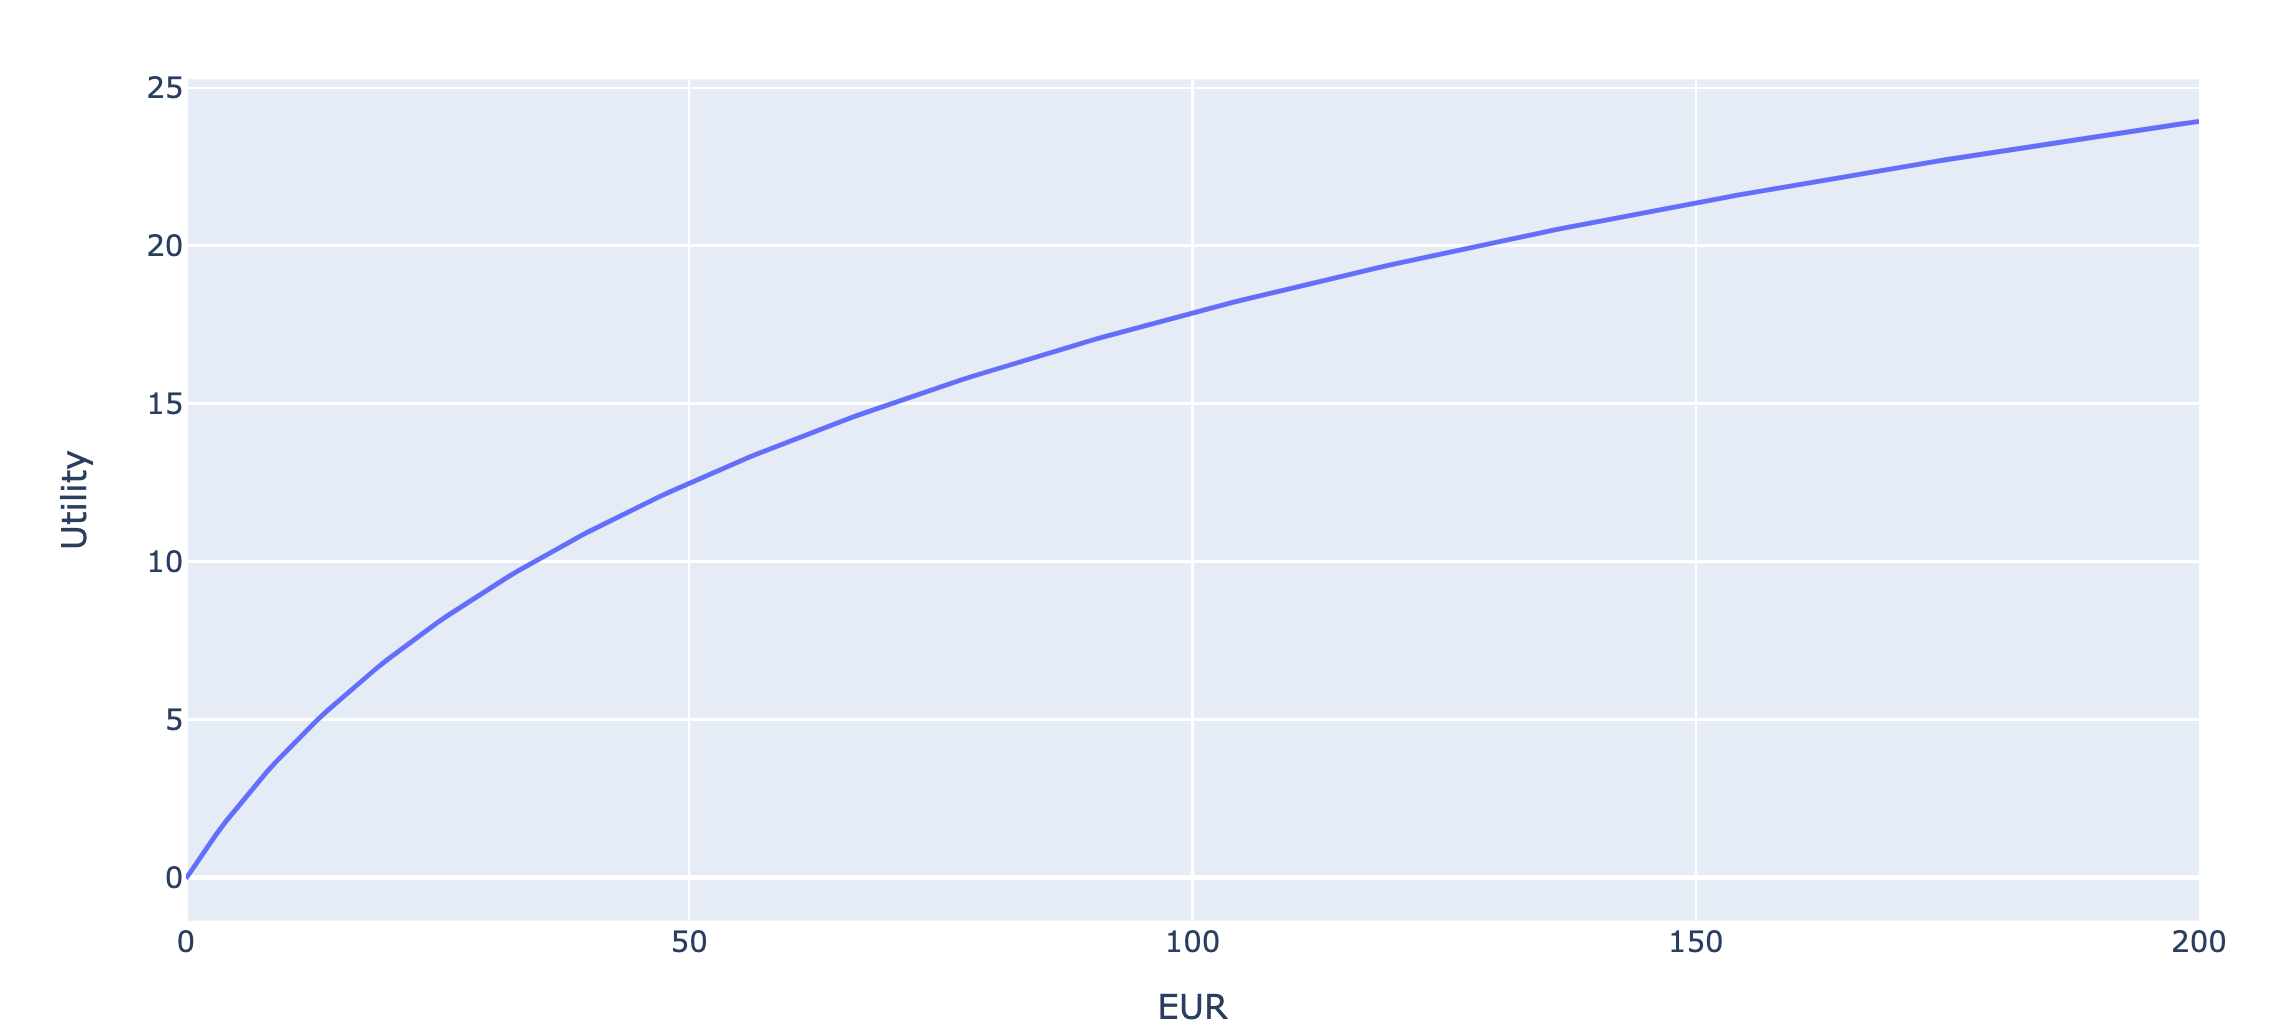
\includegraphics[scale = 0.205]{Images/UF.png}
		\caption{An example of a utility function of a risk-averse decision maker.} 
		\label{fig:UF}
	\end{center}
\end{figure}





\chapter{Valuation - State of the Art}\label{chapter:Economics}
This thesis is built on two main theoretical pillars. The first, described in the previous chapter, is the SDT. The second is the project valuation principles of corporate finance \cite{BerDeM:09}, an overview of which will be presented in this chapter. 

First, we will define the necessary project valuation terminology that will be used throughout the thesis. 

Then, we will describe the industry standard for project valuation, which is the idea of \textit{discounted cash flow} (DCF) and the corresponding metric called the \textit{net present value} (NPV). Together with NPV, we also present a new useful tool for the project's capital management called the \textit{present cash equivalent} (PCE). In addition, we recall the risk-aversion of investors. 

At the end of this chapter we will look at an advanced project valuation technique called the \textit{real option analysis} (ROA), which is based on the financial options valuation ideas. 

\section{Terminology}\label{sec:Terminology}
Let us now introduce the project valuation terminology used in this thesis. 

\paragraph{Process}
	A process is understood as the production, purchase and trade of goods or services, driven by the supply of inputs and demand for outputs.


\paragraph{Project}
	A project is defined as a sequence of actions that realize the implementation or innovation of a process, purposefully allocating existing sources to increase the economic value of a process in question.  

\paragraph{Project's free cash flow}
	The incremental effect of a project on the firm’s available cash is the project’s free cash flow (FCF) \cite{BerDeM:09}.

\paragraph{Economic value}
	An economic value of a project is understood to be in the future free cash flows. In this thesis, the economic value of a project is the amount of cash to which the investor is logically indifferent to having in comparison to the future cash flow vector. 

\begin{remark}
	The indifference is in this thesis understood in the presented concept of PCE, which incorporates the problem of project's financing in addition to the time value of money already covered by the NPV. 
\end{remark}

\paragraph{Optimal project}
	The goal of each project is to increase the economic value of a process. A project, if such exists, is called an optimal project if the additional economic value is maximal given the set of possible projects. 
\paragraph{Risk averse investors}
		A risk-averse investor is an investor, who prefers a low-volatile investment despite its lower expected return. 

\begin{remark}
	According to the observations made in \cite{BerDeM:09}, there is a positive correlation between the volatility of an investment and its average profit. This correlation is being explained by the risk aversion of investors, who keep investing in assets with a lower expected return. This phenomenon, also well documented in psychological publications\footnote{E.g., \cite{HolLau:05}, where it is observed that people value the uncertain rewards below their expected value}, has a link to the concept of utility from SDT discussed in section \ref{sec:utility}. 
\end{remark}


\section{Net Present Value}\label{sec:NPV}
The \textit{net present value} (NPV) is an industry-standard valuation metric used in capital investments. Its computation is simple and it respects the time value of money by an exponential discounting of the FCF by a constant rate $r$ (usually a risk-free interest rate). The exponentially discounted elements  $c_t, t \in \{1,...,|c|\}$ of a FCF vector $c$ form a \textit{discounted cash flow} (DCF) vector, and their sum is the NPV of $c$: 

\begin{equation}
NPV(c) = \sum_{t \in \mathbf{T}} \frac{c_t}{r^t}.
\end{equation}

There are deep economical reasons for the usage of this valuation metric in capital investment as presented in chapter 3 of \cite{CopAnt:01}. However, for the purpose of our thesis, it is worth to present a generalized version of NPV, which also incorporates the process of borrowing and repayment of cash, so called capital budgeting, which is a broad topic on its own. 

We call this new metric the \textit{present cash equivalent} (PCE) and we present it the following section. 

\subsection{Present cash equivalent}\label{sec:PCE}
The goal of the \textit{present cash equivalent} (PCE) is to value a FCF vector, while covering the problem of capital budgeting (borrowing and repayment of cash needed to proceed with the project). The usual problem of the capital budgeting needs to discuss the specific types of loans (issuing bonds, shares, taking mortgages, etc.), their different interest rates and the repayment structure. This certainly reflects the reality better, however it brings a significant overhead to the project valuation problem. 

This is why we present PCE, which incorporates the costs and the usually complex borrowing structure of the capital budgeting based on two assumptions. First is that there is a possibility of a \textit{fully liquid loan} financing with a constant interest rate $r_b$. 

\begin{definition}(\textbf{Fully liquid loan})
	A fully liquid loan (FLL) with an interest rate $\emph{r}_b$ for $\emph{n}$ periods is a loan, the initial principal of which changes after each predefined period as follows:
	\begin{itemize}
		\item If the borrower needs to borrow more money $\emph{m}$, the principal from previous period increases by the interest rate factor $1+\emph{r}_b$ and the $\emph{m}$ is added to the principal.
		\item If the borrower repays the amount of money $\emph{m}$ in a given period, the previous principal increases by the interest rate factor $1+\emph{r}_b$ and the $\emph{m}$ is subtracted. 
	\end{itemize} 
	
	The fully liquid loan ends in two scenarios. Either the principal was fully repaid in some period $t\leq n$, or it was not, the borrower is unable to pay back and defaults on the FLL. 
\end{definition}

\begin{remark}
	A fully liquid loan is a simplification of a mortgage, where the borrower is not obliged to follow a predefined payment calendar and has more flexibility even to the extend of borrowing more money. It is an idealistic representation which in real life would need to impose limits preventing the increased probability of borrower's default.  
\end{remark}

\begin{example}
	Investor borrows 1M for a new factory with a FLL with $r_b= 5\%$ for the maximum of $n=5$ years. He repays all his FCF, which is 400k in all years except of year 2. The second year ended up in a loss of 100k which investor borrows based on the ideas of FLL. This results in the following vector of principal in year 0 to year 5\footnote{The figures from year 3 are rounded to one decimal place.}:
	\begin{equation}
		[1M, \ 0.65M, \ 782.5k, \ 421.6k, \ 42.7k, \ 0].
	\end{equation}
\end{example}

The second assumption for the concept of PCE is the ability to invest money with a constant risk-free interest rate $r_r$. 

When the investor can take advantage of both the FLL and the ability to invest money with risk-free interest rate, we argue that there is only a single amount of cash, to which the investor should be indifferent to having, instead of a given FCF vector, thus making it the present cash value of such FCF vector. 

For the purpose of PCE, let us also prepare the notion of the so-called \textit{responsible manager} (RM). RM's task is to reinvest the positive balance (with the rate $r_r$) and borrow more funds in case of a negative balance for the rate of $r_b$. 

We represent this behavior by the RM function, where the constant rates are not explicitly denoted but rather implicitly assumed: 

\begin{equation}
RM(b) = 
\left\{
\begin{array}{ll}
b\cdot(1+r_r)  &  \mbox{if } b\geq 0 \\
b\cdot(1+r_b)  & \mbox{otherwise}
\end{array}
\right.
\end{equation}

Then, based on the two assumptions, we model the behavior of $RM$ on a given cash flow vector $c = \{c_0,...c_t\} \ t \in \mathbb{N}$ as: 

\begin{equation}
RM(c) = RM(...RM(RM(c_0)+c1)...+c_t). 
\end{equation}

The amount of $RM(c)$ represents the amount of money at time $t$ obtained from the cash flow vector $c$ and a logical money management. Then, the PCE(c) can be finally derived as: 


\begin{equation}
PCE(c) = 
\left\{
\arraycolsep=5pt\def\arraystretch{1.5}
\begin{array}{ll}
\frac{RM(c)}{(1+r_r)^{t}}  &  \mbox{if } RM(c)\geq 0 \\
\frac{RM(c)}{(1+r_b)^{t}}  & \mbox{if } RM(c) < 0 
\end{array}
\right.
\end{equation}


representing the logic that having PCE(c) at time $t =0$ would result in the same outcome at time $t$. Thus, an investor should be logically indifferent to obtaining $PCE(c)$ now and $c$ by its parts at different times. 

\begin{remark}
	Based on the straightforwardness of the PCE  computation, we argue that for each FCF vector, a unique PCE equivalent always exists. In the remainder of the thesis, we will understand the value of an FCF vector to be its PCE value. 
\end{remark}

\begin{example}
	Let us for the illustration value the following cash flow vector $c = [-200,100,100,100]$, which represents an initial loss and three constant follow-up profits. Assume that $r_b=10\%$ and $r_r=2\%$. Then the $RM(c) = 80.16$ and the $PCE(c) = 75.64$\footnote{Both values are rounded to two decimal places.}. For comparison, the $NPV(c) = 88.39$.
\end{example}

\section{Financial Option Valuation}
There exist two types of financial options, calls and puts. 
\begin{definition}(Call option)
	A call option gives its owner the right to buy stock (or a commodity) at a specified exercise or strike price on or before a specified maturity date. If the option can be exercised only at its maturity date it is known as European call, in other cases the option can be exercised at any time before its maturity date and it is then known as American call \cite{BreMye:12}.
\end{definition}

\begin{example}
	One share of Tesla stock is traded at $\$700$ at the moment (30.5.2021). An European call option with a strike price of $\$2500$ with a maturity date of 1.1.2022 costs $\$1.25$. An investor buys this option and two things can happen on 1.1.2022. First, more probable case is that the Tesla stock price will be lower than $\$2500$ and thus, exercising the option (buying the stock at $\$2500$) would be unprofitable. Investor doesn't do anything and he lost $\$1.25$. In a second, less probable case, the stock price rises to $x>\$2500$. In this case, the investor will use his right to buy the stock for $\$2500$, which he is able to immediately sell on the market and pocket the difference $\$(x-2500)$. 
\end{example}

\begin{definition}(Put option)
	Similarly to call options, which allow the investor holding them to buy the stock or the unit of a commodity on or before the maturity date, the put option allows the investor to sell for a given exercise price. American and European puts are again distinguished by the possibility to exercise before or precisely on the maturity date. 
\end{definition}

\begin{example}
	One share of Tesla stock is traded at $\$700$ at the moment (30.5.2021). An European put option with a strike price of $\$150$ with a maturity date of 1.1.2022 costs $\$1.25$. An investor buys this option and two things can happen on 1.1.2022. First, more probable case is that the Tesla stock price will be higher than $\$150$ and thus, exercising the option (selling the stock at $\$150$) would be unprofitable. Investor doesn't do anything and he lost $\$1.25$. In a second, less probable case, the stock price drops to $x<\$150$. In this case, the investor is able to buy the share on the market for $x$ and exercise the option (selling the share for $\$150$) pocketing the $\$(150-x)$ difference.
\end{example}

As outlined in the first chapter, the idea of options and option trading dates back to 17th century. However, the motivation for a proper option valuation technique came with the increased adoption of derivative trading after WWII. 

The famous 1973 article from Black and Scholes \cite{BlaSch:73} describes today's standard tool in the financial option valuation - the BSM model. 

\begin{remark}
	The M in BSM model stands for Merton, who expanded on \cite{BlaSch:73} with his article \cite{Mer:73} and received the Nobel price together with Scholes.
\end{remark}

In what follows, we will present the BSM model in the form of a theorem \cite{BodKan:04}. In addition, we will offer an opinion that should summarize the idea of the BSM model in few sentences. 

\begin{theorem}(BSM model)
	The Black-Scholes-Merton option valuation model says that if the following list of assumption is satisfied:
	\begin{itemize}
		\item risk-free interest rate and volatility\footnote{A variance of asset price understood as a random variable.} of the underlying asset are constant;
		\item the underlying asset pays no dividends and its price is continuous;
		\item the asset price evolves according to a log-normal process;
		\item the markets are efficient - the no-arbitrage principle holds;
		\item the option is of the European style;
		\item there are no commission or service charges;
		\item market is perfectly liquid\footnote{The investor is able to buy and sell any amount of the asset at any time and and as frequently as he wishes to.};
	\end{itemize}
	
	then based only on the knowledge of time to maturity $T$, option's strike price $K$, the current price of underlying asset $S$ and its volatility $\sigma$ the value of a \textbf{call}\footnote{Similar equation holds also for put options.} option can be computed as: 
	\begin{equation}
	C = SN(d_1) - PV(K)N(d_2), 
	\label{BSMModelEq}
	\end{equation}
	where  $PV(K)$ is the present value of a strike price $K$\footnote{Price of a bond paying K on the expiration day of the option.} and $N(d)$ is a cumulative standard normal distribution, the probability that a normally distributed variable with parameters $\mu = 0$ and $\sigma =1$ is less than $d$. Values of $d_1$ and $d_2$ are then defined as: 
	\begin{equation}
	d_1 = \frac{ln(S/PV(K))}{\sigma \sqrt{T}}+\frac{\sigma \sqrt{T}}{2},  \quad
	d_2 = d_1 - \sigma \sqrt{T}
	\end{equation}
\end{theorem}

\begin{remark}
	The option's value is positively dependent on the volatility and the time to maturity. An increase in these parameters leads to a higher option value. On the contrary, the rise in the current stock price or strike price of the options lowers an option's value. 
\end{remark}

From the combination of remarks about the BSM model from authors like \cite{BodKan:04} and \cite{Ros:11} we formulate our own remark of what does the BSM model represent. 

\begin{remark}
	The core of the BSM model, assuming that ``smooth`` conditions hold, is that we are able to derive the missing parameter $\mu$ of the asset's log-normal price model (known $\sigma$ is an assumption). Building on this, the value of an option is then the expected value of the maximum of the difference between the strike price and the asset's realized price and zero\footnote{Since when the option is not realized no further loss occurs.}, discounted by the risk-free interest rate. 
\end{remark}

Finally to illustrate the usage of BSM model we present an option valuation example from \cite{Ros:11}.
\begin{example}
	Suppose that a stock's current value is 30, the risk-free interest rate 8\% and the volatility of the stock is 0.2. Assume that all assumptions for the BSM model hold. Then the call option with strike price 34 that expires in three months has a value of 0.24. 
\end{example}


\section{Real Option Valuation}\label{sec:ROA}
As outlined in the introduction, the theory of \textit{real option analysis} (ROA), a project valuation technique inspired by the valuation of financial options, was born after the boom in publications following the BSM model in the 1970s. The first ideas presented by Myers \cite{Mye:77} are of a philosophical nature - options (ability to make project changes) help to extract the value from a project. 

Many publications were published on the ROA topic since. Through our studies of the state of the art, we have identified three classes of authors that differ by the level of analogy with the BSM model. 


\paragraph{No analogy}
The first class is the class of the ROA founder, Myers. This class understands ROA as a useful lens for looking at the project valuation. Authors like Kassar \cite{Kas:04} and Guerra \cite{Gue:17} accentuate the value of further managerial decisions, but the valuation strategy they use is NPV with scenarios (so-called decision tree analysis (DTA)). 

\paragraph{Partial analogy}
The second class of ROA authors takes advantage of the financial option valuation's core property, which is the no-arbitrage principle. Based on this principle and further assumption of replication portfolio existence, this class of authors, represented by, e.g., Guthrie \cite{Gut:09}, Thoma \cite{Tho:19} and Ryu \cite{Ryu:17}, derives so-called risk-neutral probabilities, which are then used for modeling of project's internal variable of the cash flow functions\footnote{In the majority of cases the binomial models are used.}. 

Because we find this type of approach to real options the best and because we build on and respect the work of Guthrie \cite{Gut:09}, \textbf{this approach is the one considered as representative of the term ROA. }

Another notable author in this class is Vollert \cite{Vol:03}, who goes deep into details, building a modeling framework which allows the implementation of complex conditional options. Vollert's publication is very advanced, using, for example, stochastic differential equations, which might be an obstacle for practitioners and real-world applications.  

\paragraph{Full analogy}
The final class of authors describing the ROA principle understands it as a complete analogy to the BSM model for the financial option valuation. This class of authors is predominantly represented by voluminous economic textbooks, e.g., Berk and DeMarzo \cite{BerDeM:09}, Brealey \cite{BreMye:12}, or Crundwell \cite{Cru:08}\footnote{Crundwell also discusses the partial analogy approach in detail.}. 

A complete analogy means to identify all parameters of a financial option with parameters of given investment. For example in \cite{BerDeM:09} the following identification table is presented: 


\begin{table}[H]
	\begin{footnotesize}
		\centering
		\renewcommand{\arraystretch}{1,2}
		\label{Tab:BSModel}
		\begin{tabular}{|l |r|}
			\hline	
			\textbf{Financial option}& \textbf{Real option} \\ \hline
			Stock price& Current market value of an asset \\ \hline
			Strike price& Upfront investment required	\\ \hline
			Expiration date& Final decision date \\ \hline
			Risk-free rate& Risk-free rate\\ \hline
			Volatility of stock & Volatility of asset value \\ \hline
			Dividend\footnotemark & FCF lost from delay \\ \hline
		\end{tabular}
		\caption{Identification of financial option parameters as parameters of a real option (investment opportunity). \cite{BerDeM:09}. }
	\end{footnotesize}
\end{table}
\footnotetext{In this example from \cite{BerDeM:09} the analogy is made with a generalized BSM formula for stocks with dividends. When we set dividends equal to 0, the analogy holds with the original BSM model as presented above.}

Another example published by Quélin \cite{Que:10} describes a telecommunication company valuation with the same one-to-one identification of BSM model parameters. 

By focusing on the complete analogy, the authors of this class strictly limit the application scope of their approach. One of the problematic assumptions (that is in the partial-analogy class solved by the CAMP model\footnote{Capital asset pricing model - for details please see \cite{Gut:09}.}) is that there exists a market tradeable replicating portfolio of the asset we want to evaluate. Another limitation is that this approach considers only one possible action, which is usually to invest in the project now or later\footnote{Timing option in Guthrie's terminology.}. 

\vspace{1em}


As explained in the \textit{partial analogy} paragraph we base our understanding of ROA on Guthrie's work. A rigorous definition of ROA as used in this thesis will be presented in the beginning of the following chapter. 


\chapter{Project Valuation Revisited from the SDT Perspective}
In this chapter, we develop the core idea of this thesis. The idea is to take the project valuation problem as defined in ROA, reframe it as a Markov decision process and then use the SDT techniques (such as the approximate dynamic programming) to solve it while preserving the business-specific concepts of the project valuation, such as time value of money and risk aversion of investors. 

We begin by clarifying the meaning of the term project valuation as is used in the ROA publications, and we identify the main limitations of this approach.

Next, we focus on the identification of the project valuation in terms of the SDT framework. We define all the relevant sets and functions to be able to talk about project valuation as a structured problem of decision making under uncertainty. 

The remainder of this chapter is reserved for the incorporation of the business-specific concepts to the model, namely the time value of money and the risk aversion of investors. 


\section{Project Valuation - Problem Definition}
To be able to talk about the project valuation rigorously, we need to define what a \textit{project} is and what we mean by its \textit{valuation} in ROA. The inspiration for these definitions comes from examples and used rhetoric in the ROA publications, namely \cite{Gut:09}, \cite{Vol:03} and \cite{AmrKul:98}. 

None of the publications that we have studied goes into detail to define a project as a collection of mathematical constructs, as, for example, SDT does with MDPs. Guthrie in \cite{Gut:09} opens with three initial examples of a project and in each chapter adds a new real-life investment opportunity. This investment opportunity is presented in such a way that it is clear what the project is, what its parameters are, and what metric is being optimized by the investor. 

In other publications like Vollert's \cite{Vol:03} and Kulatilaka's \cite{AmrKul:98},  a definition of a project is also not given. Rather, it is assumed that the used terms \textit{project}, \textit{capital investment}, or \textit{investment opportunity} are clear. 

It is worth noting that a definition of project \textit{valuation} is also not deeply discussed in the ROA books. We feel like the term of valuation is assumed to be clear and is always represented by the expected NPV. 

As outlined above, nothing like a clear mathematical definition of a project valuation is presented in the ROA publications. However, the used rhetoric is similar, and we strongly believe that the project valuation in the ROA field can be summarized as: ``Determining the amount of value that an investor is able to create with actions that can be considered as a part of one project\footnote{Defined as in section \ref{sec:Terminology}}, measured by the  metric of expected NPV with a special non-axiomatic determination of the discount rate.``

Now that the position of ROA to project valuation is clearer, we can follow with its interpretation in the SDT framework.


\section{Project Valuation in the Statistical Decision Theory Framework}
Trying to solve the project valuation task as a statistical decision problem means, first and foremost to identify all the necessary parts of the SDT framework in the ROA formulations. This is not a particularly hard task given the rather loose definition given above. 

After this identification, the standard tool of SDT, dynamic programming (or potentially approximate dynamic programming), can be used to solve the valuation problem. 

Solving a valuation problem in SDT means in our case to define it as MDP, which consists of two parts. First, there are three sets: the time set $\mathbf{T}$, the state set $\mathbf{S}$ and the action set $\mathbf{A}$, which describe the structure of the MDP. The second part consists of two functions: transition probability function $p$ and reward function $r$, where $p$ is responsible for describing the project's stochastic evolution and $r$ for informing about the value gains in each time epoch.

In the following sections, we will focus on each of these five important building blocks in detail. To better illustrate each of the building blocks, and to prepare the ground for the experiment, an example concerning the valuation of a gas power plant is presented. 

\subsection{Time sets}
Even though the SDT theory is capable of handling infinite time horizons and continuous-time modeling, these sophisticated formats are not needed for the valuation of real-life projects. The time dimension of a project can be reasonably described by a discrete set with a known finite horizon, which is valid for two reasons. 

First is that observing new information and making impactful decisions by the project's manager is not done continuously at all times but discretely after some practical time intervals. No manager changes the course of a project ten times a day\footnote{This thesis does not focus on the individual management of the internal processes of a project, but rather on managerial decisions that modify the project in a major way.}. 

The second reason is that managers do not think about projects as ever-lasting. Potential profits after a certain time threshold are neglected. This is given either by the finite-lifespan nature of the projects (gas power plant lifespan) or the extreme uncertainty in the modeling of FCFs (and their equivalent is present values) in the far future. To have a good model of the project's FCF in 100 years is wishful thinking. 


Time intervals in our model reflect the frequency of influential management meetings at which the project's course can be significantly changed, e.g., week, month, or quarterly intervals. This notion is further supported by its usage in ROA publications. 

\begin{example}
	Monthly decision time intervals in a duration of gas power plant lifespan, say 25 years. The time set is then $\mathbf{T} = \{0,1,2,...,300\}$.
\end{example}

\subsection{State sets} Defining the state set $\mathbf{S}$ in a project valuation problem means finding a list of relevant, measurable parameters for both the project and its environment. A state $s \in \mathbf{S}$ is then a vector of elementary states of such individual parameters. 

The state set $\mathbf{S}$ can be constant, meaning that the same parameters are measured in each time epoch. However, it might also be useful to think about dynamic state sets in time $\mathbf{S_t}$, $t \in \mathbf{T}$, where for some particular reasons, the structure of a problem changes in time\footnote{There are more or less relevant parameters to measure.}.

It is worth noting that there are usually some elementary states that are influenceable by the managerial actions and some that are not. This classification is not reflected in our notion. 

In our models, each elementary state is understood as a random variable, the probability distribution of which is conditioned on the previous state and the last action taken. This probability is described with the transition probability function $p$, which is discussed in detail below. 

\begin{example}
	Relevant features for a gas power plant project might be, for example, price of gas, price of CO2 allowances, price of power, installed capacity of the plant, or debt to be repaid. The first three elementary states would then be considered uninfluenceable by investor's future actions, while the last two would not. 
\end{example}


\subsection{Action sets}
In SDT structure, the action set  $\mathbf{A}$ is usually understood as an actual set, however in the format of project valuation, we find it better to represent it as an action function $a$, whose parameter is a  given state $s_t \in \mathbf{S_t}$ and output is a set of possible actions $\mathbf{A_{s_t}}= a(s_t)$. 

This is because possible managerial actions are most of the time strictly conditioned on the current state of the project. Only a small subset of all possible actions might be actually taken in a given state. 

In ROA publications, the term \textit{options} is used to describe possible managerial actions both current and future. Even though we believe that this terminology helps with understanding that the possibility of future managerial action has value, we do not embrace a notion of future actions or the term \textit{options} since it is not consistent with the SDT terminology. 

The advantage of the SDT approach in contrast to ROA is that there is no theoretical  complication in adding an arbitrary amount of actions of any type (as classified in ROA by Guthrie \cite{Gut:09}, for example), possibly even conditioned on one another. The only concern that needs to be reminded is that of computational complexity, where a large number of possible managerial actions decreases the ability to compute the valuation in practice. 

\begin{example}
	Possible actions for a gas power plant project might be to: build a new block of the plant, run the plant if it has some installed capacity, or wait for a better situation on the market and do nothing. 
\end{example} 

We believe that this example shows the dependency of possible actions on a given state and why it is thus better to use the function notion $a(s_t)$.

With the definition of action function, we have defined the general structure of a project, boundaries within which the project will evolve. Now, we will study the rules that guide the evolution and metrics that measure the value created. 

\subsection{Transition probability functions}
Given the nature of projects, the evolution from one state to another is stochastic. In this thesis, we want to model the project as MDP, and thus, the probability distribution of the next state, described by the transition probability function, is conditioned only on the previous state and the last action taken. In mathematical notation: 
\begin{equation}
	p(s_t|a_{t-1}, s_{t-1}).
\end{equation}

In this thesis we consider states values as a realizations of discrete or continuous random processes, described by conditional probability mass or density functions, respectively. Furthermore, as we will model each elementary state by a different distribution, we need to be able to compute the overall probability of the future state given the elementary state distributions. 

To make things simple, we assume individual elementary states to be represented by independent variables, and thus the probability (or probability distribution) of the next state is a product of the elementary probabilities\footnote{Combination of discrete and continuous variables as elementary state results in continuously distributed global state (and thus a probability distribution).}: 

\begin{equation}
	p(s_t|a_{t-1}, s_{t-1})=\prod_{i}p(s_t^i|a_{t-1}, s_{t-1}), 
\end{equation}
where $s_t^i$ is the i-th elementary state of $s_t$.

\begin{remark}
	It is possible that some elementary states are fully determined by the managerial action $a_{t-1}$. Such a corner case does not create a problem for the probabilistic notion above. The new elementary state $s_t^i$ is realized with probability $p(s_t^i|a_{t-1}, s_{t-1})=1$.
\end{remark}

It is clear that in the majority of real-life projects, determining or estimating this transition probability function is a challenging but crucial task. Decisions will be made based on its values increasing or decreasing the value of a project. 

The approach of ROA authors to the modeling of these probabilities varies a lot. Some authors like Guthrie \cite{Gut:09} or Amram \cite{AmrKul:98} use the no-arbitrage principle to determine the probabilities of their binomial models. Some authors, like Kulatilaka \cite{KulTri:94}, use the principle of insufficient reasons\footnote{Even though they do not call it that way.}, where they assign 50\% probability to movements in both directions of their binomial models. Some authors, like Guthrie \cite{Gut:09} and Vollert \cite{Vol:03}, also offer a more elaborate statistical modeling of the probabilities. 

Some details of how does SDT approach the estimation of $p(\cdot)$ will be discussed later in section \ref{sec:probability}, however, we must note that the actual estimation of these probabilities is beyond the scope of this thesis.


\begin{example}
	The evolution of a gas price can be modeled as a lognormally distributed random variable, with $\mu$ being the previous epoch's gas price and $\sigma$ an estimate, for example based on historical data. 
\end{example} 



\subsection{Reward functions}
The final part of modeling the project valuation as MDP is the reward function. Its purpose is to assign a numerical value to the state realization $s_t$ given the previous state $s_{t-1}$ and last managerial action $a_{t-1}$, mathematically: 

\begin{equation}
	r(s_t,a_{t-1}, s_{t-1}).
\end{equation}

As discussed in section \ref{sec:NPV}, the notion of \textit{value} is complicated. In our case of project valuation, this value is represented by the FCF. Thus, the first approximation of the entity to be maximized is the expected cumulative FCF, which usually consists of expenses resulting mostly from immediate managerial actions and income, the amount of which tends to result from the environment (supply and demand for products or services) conditioned on a previous action or action sequence. 

However, as the economic theory guides us, this approximation is insufficient due to the clear preference in having money now instead of later (time value of money) and the fact that investors do not value uncertain FCF the same as their expected values (risk aversion of investors). Both of these phenomena lead us to adjust the metric that is to be optimized by the optimal strategy.

The details of this alternation, driven by the two phenomena, will be deeply discussed in the following sections \ref{sec:time_value_of_money} and \ref{sec:risk_aversion}. For now, let us simply declare that the optimal strategy will be derived from a generalization of expected cumulative FCF, respecting the individual risk preferences, borrowing, and risk-free investment opportunities of the investor. 


\begin{example}
	The reward function of a gas power plant is driven by its ability to make money by transforming the gas and CO2 allowances into electrical power. The initial expenses for building the individual blocks result in extreme negative rewards (driven by the action of building). At the same time, the profits are made as a multiple of installed capacity and the difference of input costs plus fixed costs and the revenue from selling the electricity (conditioned on the action of running the plant). 
\end{example}

\bigskip

This paragraph concludes the basic identification of sets required by the SDT framework. In the next section, we will focus on the solution to the project valuation problem in detail. We will discuss the sources of transition probability function, the actual incorporation of the time value of money, and the risk aversion of investors into the model. 

\section{Solution of the Project Valuation as a SDT Problem}
In the previous chapter, we have focused on the basic structure of a project valuation understood as MDP. In this chapter, we go deeper and focus on the details of the actual solution of such valuation problem. 

We begin this section by looking in detail at the estimation of the transition probability function $p$. We outline how the SDT can not only incorporate the ideas of ROA but also help with more advanced estimation techniques. 

Then, we continue with the incorporation of the business-specific concepts - time value of money and risk aversion of investors in the form of utility maximization principle and the notion of PCE. We focus on implementation details with an accent on applicability by real-life investors. 

Finally, the last part of this section addresses the computational complexity problems of classical dynamic programming, proposing an ADP class algorithm identified as the best fit for a project-valuation-style MDPs. 


\subsection{Probability}\label{sec:probability}
In this thesis, we focus on real-life projects. Such projects are, by their nature stochastic, and except for some edge cases, the laws guiding the evolution of the relevant parameters are unknown and complex. Our search for the optimal strategy is based on the assumption that we have some model estimating the future paths of the project states, and we act as if this model was the reality. In our case, the model of this evolution is materialized in the form of transition probability function $p$, where for example, one of the assumptions is the Markovian property of the states\footnote{Meaning that the probability of evolution to the state $s_{t+1}$ depends only on $s_t$ and $a_t$.}. 

There are many ways how to model $p$. Let us discuss the techniques used in ROA publications and how they can be translated into the SDT terminology. Furthermore, let us also outline the more advanced techniques that SDT can offer in this section. 


\paragraph{Risk neutral probabilities}
The idea of risk-neutral probabilities together with the binomial model is the major modeling force in the ROA publications. We observe two levels of its usage, both of which are based on the principle of arbitrage non-existence.

First, simpler approach, used by Ryu \cite{Ryu:17} or d'Amato \cite{DamZro:19}, adjusts only for the time value of money represented by the risk-free rate $r_f$, where the probability of up and down moves are computed as:
\begin{equation}
	\pi_u = \frac{r_fX-X_d}{X_u-X_d},  \quad \pi_d = 1-\pi_u,
\end{equation}
and where $X$, $X_u$, and $X_d$ are the values of the asset price now, after one up move and after one down move. These equations represent the idea that the probability of up and down moves of an asset are such that its expected appreciation is equal to the risk-free interest rate. 

The more complex equation, also adjusting for the specificity of the risk of the field we invest in, called risk premium, comes from the capital asset pricing model (CAPM). This model is used by the frequently mentioned Guthrie in \cite{Gut:09}, but also by other authors, such as Lund \cite{LunDid:17}.

This technique is presented exclusively in the context of binomial models, but it is easy to imagine its usage for their limit case, which is a variable with the Poisson distribution. 

\paragraph{Insufficient reasons}
The second widely observed modeling style in ROA publications, used mostly in addition to the binomial model, is to assign 50\% to both up and down move. This technique can be used on different levels of the model, as the final model (as in \cite{KulTri:94}) or, for example, as a helping distribution modeling a particular supportive distribution (as in \cite{Gut:09}).

It needs to be emphasized that the ROA authors do not use the term \textit{insufficient reasons} themselves. 

\paragraph{More complex models}
In more mathematical publications, we observe more complex models of the future state outcomes, for example, the normal process with dynamic parameters \cite{BenWhi:17} or \cite{AlsWan:20}, the mean-reverting process with Poisson jumps \cite{SchRob:19}, or a general \^{I}to process \cite{Vis:18}. 

It seems that these models come from authors with more mathematical than economic background and their unifying feature is the rigorous usage of random variables and continuous distributions. 


\paragraph{SDT interpretation}
Now we would like to discuss the interpretation of the ROA probability modeling techniques in SDT. The notion of risk-neutral probabilities can be approached with the framework of \textit{expert knowledge}, where the first expert is the one (usually the economist using the CAPM formula) who determines the individual variables like the risk-premium or expected market growth. In accordance with the philosophy of \textit{experts}, the second expert is the market behaving by the non-arbitrage principle, giving us the equations for risk-neutral probabilities. 

The term of insufficient reasons comes from the SDT itself, and thus, it was already interpreted above. 

The class of more advanced approach that we have discussed above is easily covered with the SDT too, because of its structure. The outputs in terms of distributions, coming either from the data or again the \textit{expert knowledge}, are easily incorporated into the SDT framework as prior (static or dynamic) probabilities.   

\paragraph{SDT innovation}
The portfolio of SDT estimation techniques is much broader than what was discussed so far. Because the probability estimation is not the main focus of this thesis, we will only outline two of the most interesting techniques. 

First is the Bayesian modeling, where each time new data are being observed, our probability model is updated by the Bayesian formula. This very influential modeling technique in SDT was not seen in the studied ROA publications, even though there is certainly a space for it. 

The second modeling strategy that we want to talk about is the consistent way of information fusion from different sources. This niche part of the SDT, lead by Kárný \cite{Kar:20}, allows for the incorporation of multiple sources of prior probabilities, for example, multiple experts, data sources, and more.

\paragraph{Summary}
To conclude, we advice to use one of two approaches to the problem of $p$ estimation. First, when a lot of information about the project is known, we have a strong case for the parameters behaving according to given smooth distributions. Additionally if we believe the market to compactly represent the expert knowledge, we prefer Bayesian updated risk-neutral probabilities. 

On the other hand, if the project is truly innovative and there is very little data to base our model on, we prefer to use a combination of expert knowledge and principle of insufficient reasons to determine the priors. 

In the end, we leave the decision of the actual modeling to the framework user, where we express the sympathy for simple models, where more ``unclear`` models, in spite of their better precision, might not be accepted by the investment board making the final investment decisions. Clearly, we do not advise using niche SDT modeling techniques like probability distribution fusion from Kárný \cite{Kar:20}. 



\subsection{Time value of money}\label{sec:time_value_of_money}
As outlined in \ref{sec:NPV}, money does not have the same value through time. This concept is one of the most important ones in project valuation and capital budgeting. The approach of the economic theory to this problem is to exponentially discount the FCF with the so-called risk-free interest rate and measure value of a FCF vector with the NPV metric. 

In this thesis, we will use the upgraded version of NPV, described in section \ref{sec:NPV} as PCE, which already accounts for the process of borrowing and reinvesting the money from the FCF vector in a sense of a \textit{responsible manager}. The ability to finance the project with a \textit{fully liquid loan} FLL and the ability to invest in risk-free asset is assumed. 

Earlier in this thesis we have denoted the expected cumulative future FCF as the first approximation of a metric that we want to maximize with our decision making. Now, we present the second approximation of the optimized entity, which is original for both the ROA and SDT\footnote{SDT theory uses exponential discounting, for example, in models with infinite time sets, however, through our study, we have not encountered the idea of discounting conditioned on a state.} world, the PCE. 

The PCE represents the amount of money the investor is logically indifferent to having now instead of a vector of future cash flows. As argued in section \ref{sec:NPV}, this value is unique and always defined. 

The following equation represents the update of the Bellman equation \ref{eq:Bellman}, adjusting the crucial step in the optimal strategy determination:

\begin{equation}
v(s_{t-1}) = \max_{a_{t-1} \in \mathbf{A_{s_{t-1}}}}\sum_{s_t \in \mathbf{S_t}} P(s_t|a_{t-1}, s_{t-1}) PCE\left(\left[s_{t-1}^b,v(s_t)+r(s_t,a_{t-1}, s_{t-1})\right]\right),
\end{equation}
where $s_{t-1}^b$ is the project's balance state in time $t-1$.

\begin{remark}
	In essence, this notion only ensures that different discounting of future cash flow is applied for cases where the project is in debt (and thus investors value the earlier cash flow more), and when its balance is already positive. In a case that $r_r = r_b$ holds for the available FLL, the NPV notion gives the same results as PCE.
\end{remark}


\subsection{Risk aversion of investors}\label{sec:risk_aversion}
As discussed above, the nature of real-life projects is stochastic. The uncertain evolution of states results in the uncertain FCFs defined by the function $r$, which has implications for the investor's decision making. 

As discussed in section \ref{sec:Terminology}, the majority of investors is risk-averse, meaning that they tend to value uncertain gains lower than is their expected value. 

We believe that this characteristic of investors is important to consider in the valuation of a project. Fortunately, the SDT theory already has a framework for coping with such skewness in reward perception called the utility theory. 

The third and final approximation of the optimized entity and the corresponding adjustment of the Bellman equation \ref{eq:Bellman} is to transform the PCE by the utility function $\mu(\cdot)$ of a given investor, which can be expressed as: 

\begin{equation}\label{eq:third_approximation}
	v(s_{t-1}) = \max_{a_{t-1} \in \mathbf{A_{s_{t-1}}}}\sum_{s_t \in \mathbf{S_t}} P(s_t|a_{t-1}, s_{t-1}) \mu\left( PCE\left(\left[s_{t-1}^b,v(s_t)+r(s_t,a_{t-1}, s_{t-1})\right]\right)\right).
\end{equation}

\begin{remark}
	Even though there are consistent methods for obtaining the utility function of individual investors, it might be hard to get them on board with the idea of utility\footnote{The investor might not have time to answer the utility questionnaire as suggested by \cite{BacChi:19}, or he might be discouraged by the idea of his own skewed perception of rewards.}. This does not present a fundamental problem for our valuation technique because we can always use the utility of the risk-neutral investor, which is unique and its usage supported by the lack of bias against uncertain outcomes. 
\end{remark}



\subsection{Approximate dynamic programming}


As mentioned in the previous sections of this thesis, the classic DP algorithm can be used for the computation of MDP's optimal strategy only with rather small cardinalities of the $\mathbf{A}$, $\mathbf{S}$, and $\mathbf{T}$ sets. This known DP problem is in literature addressed as ``three curses of dimensionality`` \cite{Pow:11}.

Real-life projects, interpreted as MDPs, are usually rather complex and hardly-ever fulfill this condition. For example, when even one measured parameter is modeled to come from a continuous distribution, the DP algorithm breaks down not only from the limitation of the actual computational complexity but also theoretically. 

It might be clear from the rhetoric of this thesis that our goal is to use the developed valuation technique in practice. That is why we want to address this problem with the goal to make the solvable class of project valuation problems as large as possible. We try to accomplish that with the \textit{approximate dynamic programming} (ADP) approach. 

From the numerous ADP techniques, we have chosen the value iteration with parameter model approximation for two main reasons, both of which originate in project valuation's fundamental characteristics. 

First is that the real-life projects tend to have large state spaces (even uncountable), while on the other hand, the action set is usually limited. We cannot ask the investor to choose between 10 000 actions, for example. This argument supports the choice of value iteration over a policy iteration class of ADP. 

The second reason is that we usually have a good intuition of what precisely in the given states of the project ``makes money``. This allows us to build a good approximation function $f$ with reasonable parametrization, capturing the most important parts of the model. 


It needs to be clarified that even though we believe that our approach is generally the best, regarding the mathematical complexity, its precision and clarity, there might be better ADP algorithms for individual projects the reader intends to value. 

\subsection{Summary}
This subsection summarizes the core idea of this thesis. 

First, we have presented the interpretation of the project valuation problem as a MDP. We have defined all its important parts in detail and offered examples for clarity.

Then, we have adjusted the Bellman function \ref{eq:Bellman} to respect the business-specific concepts with the notion of PCE (respecting the time value of money and incorporating the capital budgeting problem) and utility function (the interpretation of investors' risk aversion).

In the end, we have advised the best ADP algorithm that copes with the problems of computational complexity of the usual DP solving algorithm for non-trivial projects that can naturally be used with the adjusted Bellman equation \ref{eq:third_approximation}.




\chapter{Valuation of Simple Flow Businesses}\label{chapter:Experiment}
In the previous chapter, we have presented an algorithmic approach to a project valuation based on the SDT framework and its ideas. Now we want to illustrate the actual usage of this algorithmic approach on a chosen class of projects. 

We have chosen the class of projects that can be labeled as an investment in \textit{simple flow business} (businesses that can, for the valuation purposes, be described by a straightforward transformation of input to outputs process). This class is characterized by a large outflow of money at the beginning, which is used for building the business (or its first functional part) and a small but long-term positive FCFs driven by the difference in the price of inputs and outputs and the further managerial decisions. 

This class choice is supported by its appropriate level of complexity, which allows demonstrating the power of the proposed algorithm while at the same time not being too complicated. It is also a type of project that is substantially represented in the world of capital investment. 

We could write this whole chapter using a general description of the chosen project class, however, we believe that using only one specific representative will result in a clearer picture of the situation. 

Our choice of the representative - an investment into a gas power plant - is based on three grounds. First, there is certainly an influence by Guthrie's example of a similar valuation problem \cite{Gut:09}. Second, as we will see, this valuation problem has reasonable dimensions that allow for a good presentation of the valuation algorithm. Lastly, the author of this thesis has proven domain knowledge based on his short but intensive work experience in the field of electricity trading. 

In the first part of this chapter, we will describe the valuation problem in detail. 

In the second part, we will compare the PCEs of three baseline operational strategies and the optimal one derived from the valuation algorithm. Furthermore, we will study the influence of the increased volatility of prices on the final valuation. From what we have learned about the value of real options, the project's value should increase together with the volatility increase. 

It needs to be emphasized that the aim of this experiment is to present the valuation algorithm, observe and describe its possible shortcomings and support its viability, not to prove any other theorems or ideas about project valuation.


\section{General Settings of the Experiment}
First, let us clarify what we mean by the phrase \textit{investment in the gas power plant}. We are positioning ourselves in the role of an investment analyst of a large utilities company\footnote{Companies that generate electric power usually provide also gas, water, sewage or other basic services.} whose task is to evaluate the value of building and managing a new gas power plant. 

For simplicity, we are considering building only one or two 200MW blocks, the lifespan of which ends 25 years from now, disregarding the time they were built  \cite{Car:12}. We assume that each block's price is 65M EUR, which is a rough estimate based on \cite{Bre:10}. 

We model the power plant to be managed in a monthly pattern. Its power is being sold by monthly contracts at the beginning of each month when the needed gas and CO2 inputs are also modeled to be purchased. This results in certain FCFs that are assumed to be obtained immediately after taking one of the allowed actions. As was indicated earlier in this thesis, we do not want to go deep into the plant management and its internal processes. 

The project's financing is done by a FLL with $r_b =6\%$ and $r_r=2\%$. The reality of having non-zero initial funds is reflected in the existence of the corresponding elementary state. 

Now that we have clarified the project that we want to value, we can proceed with its precise definition in the MDP format. 


\subsection{Time set}
As outlined in the introduction of this chapter we assume that the lifespan of the project is 25 years disregarding the epoch in which the plant is built. The plant management is done on monthly basis and thus the time set is defined as:
\begin{equation}
\mathbf{T} = \{0,...300\},
\end{equation}
where the epoch $300$ is understood as the final epoch, where no actions can be made, and no FCF can be obtained. 


\subsection{State set} 
The state set needs to consist of the smallest number of relevant parameters that enable us to model the process of building and running the power plant and capturing the FCF and its derived metrics for the project. 

As such, we identify five elementary states as parameters describing:
\begin{itemize}
	\item the price of gas - $s^1$;
	\item the price of CO2 allowances - $s^2$;
	\item the price of power  - $s^3$;
	\item number of power plant blocks built - $s^4$;
	\item cash balance of the project (modeling the debt) - $s^5$;
\end{itemize}
in the start of each time epoch.

The states of the state set are defined as having a constant length since there is no significant change in relevant parameters through project's lifespan. 

Mathematically the state set $\mathbf{S}$ is defined as: 
\begin{equation}
	\mathbf{S} = \{(s^1,\dots,s^5)|s^i \in \mathbf{S^i}, \ i \in(1,...,5))\}, 
\end{equation}
where $\mathbf{S^i}$ represents the limitation of the individual elementary states. These limitations will be in detail discussed now. 

For the states representing prices, $s^i, i \in \{1,2,3\}$, we define: 
\begin{equation}
	\mathbf{S^i} = \mathbb{R}_{0}^+.
\end{equation}

The next elementary state, $s^4$, represents the number of blocks built, simply:
\begin{equation}
\mathbf{S^4} =  \{0,1,2\},
\end{equation}

The final elementary state, representing the financial balance of our project, is then allowed to have any real value:
\begin{equation}
	\mathbf{S^5} = \mathbb{R}.
\end{equation}

The defintion of the state set $\mathbf{S}$ represents the problem structure, the boundaries within which the simulation of initial investment and further managerial actions will take place. 


\subsection{Action function}
In this experiment, we consider four managerial actions. They could be understood as two-dimensional, where the first dimension represents the act of running the installed capacity of the plant (if one exists), whereas the second manages the action of building new blocks. However, we have decided to use the following one-dimensional encoding:
\begin{itemize}
	\item 0 - do nothing (don't build a new block and do not run the production),
	\item 1 - run the existing installed capacity,
	\item 2 - run the existing capacity and build a new 200MW block,
	\item 3 - build a new 200MW block.
\end{itemize}

As discussed earlier in this thesis, certain actions are available only in certain states. The state that determines what actions are possible is exclusively the elementary state $s^4$ describing the number of blocks built. 

In the following list, we express the possible action set as a result of the action function in all possible elementary states $s^4$ with a short explanation of its meaning. 

\begin{itemize}
	\item $a(s^4=0) = \{0,3\}$ - when nothing is built, we can build the first block or do nothing and wait. 
	\item $a(s^4=1) = \{0, 1, 2, 3\}$ - when only one block is built, all actions are possible. 
	\item $a(s^5=2) = \{0,1\}$ - when two blocks are built, the building actions are not possible. 
\end{itemize}


\subsection{Transition probability function} 
The best way to describe the model of evolution from one state to another is to assume the independence of random variables representing the individual elementary states. This allows computing the probability of state transformation as a product of transition probabilities of the individual states: 
\begin{equation}
	p(s_{t+1}|s_t,a_t)= \prod_{i = 1}^{5} p(s_{t+1}^i|s_t^i,a_t).
\end{equation}

In our example, there are five elementary states, where the ones representing prices of gas, CO2 allowances, and power are modeled in the same way. The other two elementary states are deterministic but differ in the dependency on the previous state and action. Let us now describe the evolution of the individual elementary states in detail.

\paragraph{Commodity prices}
The prices of gas, CO2, and power are modeled by a Geometric Brownian motion, the model used in the BSM model and other publications like \cite{Vol:03}.

The probability of the next elementary state is thus conditioned only on the value of the previous state as: 
\begin{equation}
p(s_{t+1}^i|s_t^i) = s_t^i\cdot exp\left(\left(\mu -\frac{\sigma_i^2}{2}\right)\Delta t+\sigma_i W_{\Delta t}\right)
\end{equation}
for $i \in \{1, 2, 3\}$, where $\Delta t$ represents a time fraction in years, for us $1/12$, the epoch time $t+1 =t+\Delta t$, and $W_t$ is a Wiener process with probability density function defined as: 
\begin{equation}
p_{W_t}(x) = \frac{1}{\sqrt{2\pi t}} \cdot exp\left(\frac{-x^2}{2t}\right).
\end{equation}


 To be able to model the prices, we need to present the variances $\sigma_i$ and the initial values $s_0^i$ for all $i \in \{1,2,3\}$.
 
 The initial prices that we use are inspired by the real prices of commodities that are being traded on the Intercontinental Exchange (ICE). In this thesis, we would like to avoid going into the details of plant efficiency and unit transformation. Thus we present the initial prices as illustrative and already transformed to EUR per MWh produced.
 
 Similarly, the values of individual commodity variance $\sigma_i$ are inspired by our experience with the ICE and the realization of commodity prices in recent years. However, they still remain only illustrative. 
 
 In table \ref{Table:init_values}, we can see the chosen initial prices and two triplets of volatilities, which are presented due to the second goal of this experiment, determining the influence of volatility on the value of a gas power plant project. The second triplet is chosen simply as a 20\% increase of the first. 
 \begin{table}
 \begin{center}
 	\begin{tabular}{|l |r |r |r|} 
 		\hline
 	    &	Initial price [EUR] & Volatility 1 & Volatility 2 \\  
 		\hline
 		Gas & 25 & 0.12 & 0.144 \\ 
 		\hline
 		CO2  & 10 & 0.10 & 0.12 \\
 		\hline
 		Power & 37 & 0.15 & 0.18 \\
 		\hline

 	\end{tabular}
 	\caption{Initial prices of commodities and their illustrative volatilities used in the experiment. }
 	 	 		\label{Table:init_values}
 \end{center}
 \end{table}
 
\paragraph{Installed capacity}
The evolution of elementary state $s^4$ representing the number of blocks built is deterministic and conditioned on the previous action. If the chosen action is $a = 2$ or $a=3$, representing building a new block, then the elementary state of the number of blocks increases by 1 with probability 1. If the chosen action is $a=0$ or $a=1$, this elementary state is not changed with probability 1, mathematically: 
\begin{equation}
P(s^4_{t+1}=y|s^4_t = x, a_t) =
\left\{
\begin{array}{ll}
1  & \mbox{if } x = y \land a_t \in \{0,1\}  \\
1 & \mbox{if } x+1 = y \land a_t \in \{2,3\} \\
0 & \mbox{otherwise} 
\end{array}
\right.
\end{equation}
Clearly $s_0^4=0$.

\paragraph{Balance}
The last model that needs to be discussed is the one representing the financial balance of the project, $s^5$, which is driven by the simulation of an RM behavior with $r_b = 6\%$ and $r_r=2\%$. This evolution is mathematically described as: 

\begin{equation}
P(s^5_{t+1}=y|s_t, a_t,  s_t^5=x) =
\left\{
\begin{array}{ll}
1  & \mbox{if } y = RM(FCF(s_t, a_t)+x)\\
0 & \mbox{otherwise,} 
\end{array}
\right.
\end{equation}
which means that this elementary state is deterministic, and its value $s^5_{t+1}$ is computed as a result of responsible managerial actions with the previous balance $x$ adjusted for the FCF obtained in the previous state $s_t$ given the action $a_t$. 

The actual computation of $FCF(s_t,a_t)$ will be revealed in the next section, whereas the $RM$ function can be found in section \ref{sec:PCE}. The model allows for easy interpretation of non-zero initial balance, however, in our experiment, we define $s^5_0=0$.  



\subsection{Reward function}
The FCF model in our example, and actually in all projects in the class of simple flow businesses, is fairly straightforward.

First, we account for the fixed price of maintenance $C_m$, which in our case is illustrative and defined as $C_m=6$ EUR/MW of installed capacity for each hour. 

Then, conditioned on the action of running the business, we account for commodity input costs (here gas and CO2). Finally, we add the profit from selling our product on the market, and the computation for FCF is complete. 

The mathematical expression of the sentences above can be presented as:
 
 \begin{equation}\label{eq:fcf_function}
  	FCF(s_t,a_t) =s_t^4 \cdot \Big[-C_m + I_{\{1,2\}}(a_t)\cdot (s_t^3 - s^2_t - s_t^1)\Big]\cdot 200 \cdot h_m,
 \end{equation}
 where $h_m=720$ is a constant representing approximation of hours in month, not accounting for the changes in month lengths. 

\begin{remark}
	As discussed earlier, the optimal strategy is not being optimized for the expected cumulative FCF, but rather each action optimizes the expected utility of the PCE in the current state. 
\end{remark}


\subsection{Utility function}
The chosen utility function $v$ for this example was chosen as:

\begin{equation}
\mu(x) =
\left\{
\begin{array}{ll}
-(-x) ^{0.9}  & \mbox{if } x<0,\\
x^{0.85}& \mbox{otherwise.} 
\end{array}
\right.
\end{equation}

This choice represents slight risk aversion of the investors, with an asymmetric perception of losses and gains. Its purpose is only illustrative as the details of utility function creation, its meaning,  and derivation are out of the scope of this thesis. 
 
 \section{Approximate Dynamic Programming}
 
 In preliminaries we have discussed the algorithm for modeling the value function with some general function $v_t(s) = f(s, \theta_{i,t} )$. Now, as we have defined our problem, we are able to describe the specific model for our case. 
 
 Based on the initial observations of state-utility pairs coming from the performed simulation (see algorithm \ref{alg:VFapp} step 10 and figure \ref{fig:PW_linear}) and the intuition that the FCF function, equation \ref{eq:fcf_function} gives us, we have decided to model the value function with a model of three picewise linear models with one breaking point $x_{i,t}, y_{i,t}$: 
 
\begin{equation}\label{eq:VFmodel}
	v_t(s) = \sum_{i=0}^{2} I_{i}(s^4) pw(s^3-s^2-s^1, k_{i,t}^1, k_{i,t}^2, x_{i,t}, y_{i,t}), 
\end{equation}
where $I_i$ is an identificator function of installed capacity $s^4$, and $k_{i,t}^1$,  $k_{i,t}^2$ represent the slopes of the piecewise linear function model. For a better illustration, we present an example of such model fitted to the real data in figure \ref{fig:PW_linear}.


\begin{figure}[htb]
	\begin{center}
		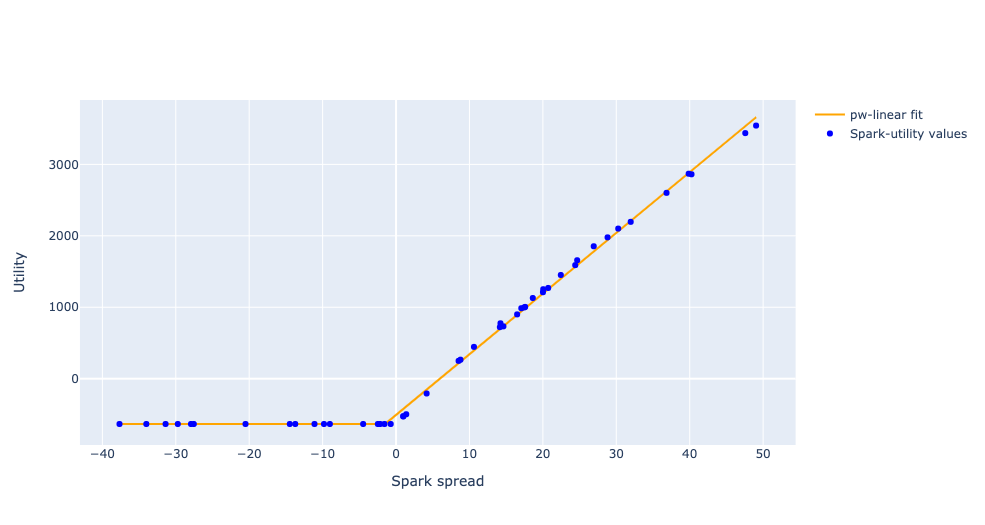
\includegraphics[scale = 0.47]{Images/pw_linear_example.png}
		\caption{Example of a pw linear fit.} 
		\label{fig:PW_linear}
	\end{center}
\end{figure}
 
 
This model effectively reflects only two variables, the installed capacity of the power plant, reflected by the choice of three models and generalized ``spark spread`` $s_t^3-s_t^2-s_t^1$, which reflects how much money is being made by running the plant with the current costs of inputs and the market price of power. 

The value function in each time epoch $t$ can thus be represented by twelve variables $k_{i,t}^1, k_{i,t}^2, x_{i,t}, y_{i,t}$ for $i \in \{0,1,2\}. $

To determine these parameters for our example, we will use the ADP algorithm of value iteration, which we describe in general by a pseudo-code in Algorithm \ref{alg:VFapp}. The important details of this algorithm are then discussed in the individual paragraphs.  

\begin{algorithm}
	\caption{ADP value iteration algorithm}\label{alg:VFapp}
	\begin{algorithmic}[1]
		\Require{$v_{300}(s)$}
		\State Prepare empty list $L$ for vf model parameters
		\For{ t $\in (299,298,...0)$} \Comment{Backward epoch induction}
			\State Prepare state sample $S_t$ \Comment{See paragraph \textit{state sampling}}
			\State Declare empty list of state utility pairs $l$
				\For{$s \in S_t$}
					\For{$a \in a(s)$} \Comment{All allowed actions in given state}
						\State\parbox[t]{.5\linewidth}{Evaluate the expected utility of an action $a $, $\mu_a$ given $v_{t+1}$ approximation} \Comment{See \textit{expected utility} paragraph}
					\EndFor
					\State Determine $\max_{a \in a(s)}\mu_a = \mu$.
					\State Save $(s,\mu)$ pair in a list $l$.
				\EndFor
			\State Fit the $(s,\mu)$ pairs from $l$ to the model described by equation \ref{eq:VFmodel}
			\State Save the fit parameters  $k_{i,t}^1, k_{i,t}^2, x_{i,t}, y_{i,t}$ for all $i \in \{1,2,3\}$ in a list $L$
		\EndFor
		\State	\Return{$L$}
	\end{algorithmic}
\end{algorithm}

\paragraph{Last VF}
For the consistency in notation, there is a need for the definition of the value function in the last epoch, where no action is possible anymore. Since the value function represents the metric of expected reward in the future, its value is 0. In our case, the $v_{300}$ is represented by the same model shown in equation \ref{eq:VFmodel} with all parameters equal to 0. 

\paragraph{State sampling}
In the third step of our algorithm, we define a state sample. This state sample serves the purpose of a reasonable coverage of the uncountable state space with a finite number of values. In this thesis, we create the sample by making samples of individual elementary states, which are then randomly put together, creating a random realization of a global state. 

In the following table, we describe the distributions out of which the elementary realizations are taken. 
\begin{center}
	\label{Table:sample_values}
	\begin{tabular}{|l |m{4cm}|} 
		\hline
		\textbf{Elementary state}&	\textbf{Distribution}  \\  
		\hline
		Gas price & Uniform (0,30) \\ 
		\hline
		CO2 price  & Uniform (0,40)  \\
		\hline
		Power price & Uniform (10,80)\\
		\hline	
		Number of blocks & $p(s^4=0)=0.3$ \newline  $p(s^4=1)=0.35$ \newline $p(s^4=2)=0.35$ \\
		\hline	
		Balance& Uniform (-60M, 60M), \\
		\hline	
	\end{tabular}
\end{center}

All the random variables are generated by the Python library NumPy, and the sample size was chosen as $|S_t|=100$.

\paragraph{Expected utility}
In step 7 of algorithm \ref{alg:VFapp}, we want to assign individual action $a$ in state $s$ the expected utility. This assignment is made with the help of the equation \ref{eq:third_approximation}, respective its part: 
\begin{equation}\label{eq:exp_util}
	\int_{s_t \in \mathbf{S_t}} p(s_t|a_{t-1}, s_{t-1}) \mu\left(PCE_{r_r,r_b}\left(\left[s_{t-1}^b,v(s_t)+r(s_t,a_{t-1}, s_{t-1})\right]\right)\right) d s_t,
\end{equation}
which was adjusted for our continuous case, changing the sum for an integration. 

To compute this expression, we use a simple numerical integration technique. Based on the state in which we are in $s_t$ and the transition probability function $p(s_{t+1}|s_t,a_t)$ defined above, we simulate chosen number of state evolutions, here $n=100$. Then the result of the numerical integration is the average of the individual utilities of PCEs of the realizations $s_t$.


\paragraph{Model fitting}
In step 10 of our ADP algorithm, the data from list $l$ are being fitted by the model described by equation \ref{eq:VFmodel}. We do this in reality by fitting three individual subsets, one for each of the plant states, by the pw linear function with one breaking point. The individual fits are done with the help of Python library lmfit, which is using the least square evaluation metric. 


\section{Optimal Strategy Performance}
Now that we have the estimation of the value function in our hands, we are able to value the project. The only thing that we need to do is to insert the chosen initial state $s_{init} = (25,10,37,0,0)$ defined above by parts into the model as $v_0(s_{init})$, which gives us the result of 388M EUR. 

Now, we want to verify the sensibility of this result by a simulation of the actual decision-making process and comparing it with some baseline strategies. Let us first define these strategies and then the simulation algorithm according to which we will compare them to the optimal strategy. 

\paragraph{Baseline strategies} 
\begin{itemize}
	\item Strategy $B_1$ builds two blocks of the powerplant in time epoch 0 and 1 and then runs them disregarding all the other factors.
	\item Strategy $B_2$ builds two blocks of the power plant similarly to strategy $B_1$, but it runs the plant only if the prices are favorable, meaning $s_t^3-s_t^2-s_t^1-C_m>0$. 
	\item Strategy $B_3$ does not build the blocks right away but waits for more favorable market states than the $s_{init}$ provides. It builds a new block only when the generalized spark price rises above the arbitrarily chosen amount of 40 EUR ($s_t^3-s_t^2-s_t^1-C_m>40$). The rule for running the installed capacity remains the same as for the strategy $B_2$.
\end{itemize}

\paragraph{Simulation algorithm}
In this paragraph, we will describe the simulation of the decision making upon which we compare the performance of our optimal strategy and the baseline strategies $B_i$, $i \in \{1,2,3\}$.


\begin{algorithm}
	\caption{Strategy performance algorithm}\label{alg:Simulation}
	\begin{algorithmic}[1]
		\Require{Strategy $B$, $r_r$, $r_b$} 
		\State Define intitial state $s_0 = (25,10,37,0,0)$
		\For{ t $\in \{0,1,...299\}$} 
			\State Determine action $a_t$ in state $s_t$ according to strategy $B$ \Comment{See \textit{determine actions} below}
			\State Compute $s_{t+1}$ realization from the transition probability function $p$ and $s_t$
		\EndFor
		\Return PCE($s_{300}^5$, $r_r$, $r_b$) \Comment{The PCE of final balance of the project}
	\end{algorithmic}
\end{algorithm}

\paragraph{Determining actions}
The general step 3 in the algorithm differs based on the type of strategy. The actions of baseline strategies are clearly defined, however, the action of the optimal strategy computed by the ADP algorithm needs to be computed again. 

The action taken in the case of the optimal strategy is determined as the action with the highest expected utility, computed as a numerical approximation of the equation \ref{eq:exp_util} with 100 numerical integration samples as before. 

\subsection{Results - initial setup} 
Now, we are able to use algorithm \ref{alg:Simulation} to compare the optimal strategy to the baseline strategies. We do this by running the simulations 3000 times and comparing the average gains (in terms of PCE) of each strategy, a Monte Carlo approach. The results of the simulations can be seen in figure \ref{fig:Results_init}. 


\begin{figure}[htb]
	\begin{center}
		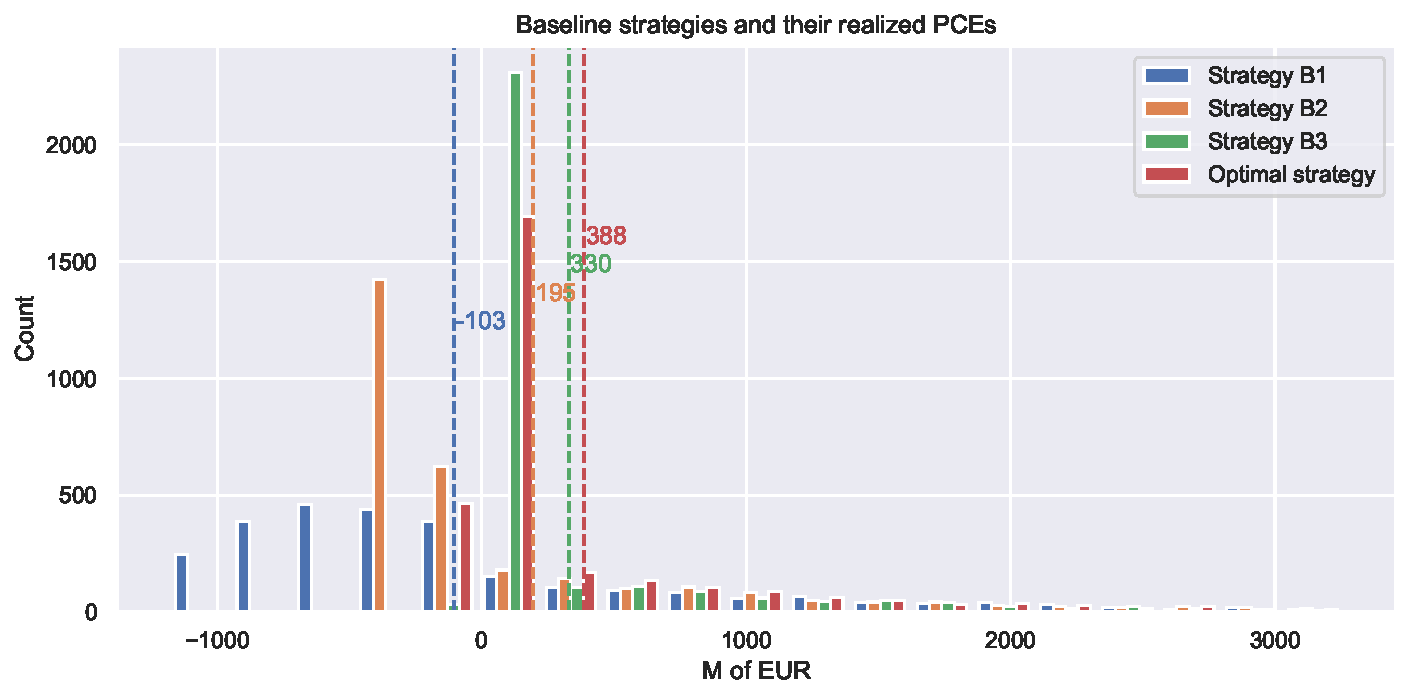
\includegraphics[scale = 0.65]{Images/MT_results_1.pdf}
		\caption{Comparison of average PCE equivalents of individual strategies, realization histograms and averages with initial settings.} 
		\label{fig:Results_init}
	\end{center}
\end{figure}



\subsection{Results - increased volatility}
The second part of the simulation is exactly the same as the first part, the only change is in increase of all price volatilities by 20\%, as can be seen in table \ref{Table:init_values}. The results of this simulation can be seen in figure \ref{fig:Results_increased}, while the comparison of individual results for both cases can be found in table \ref{Tab:Result_comparison}.
 
 
 
 \begin{figure}[htb]
 	\begin{center}
 		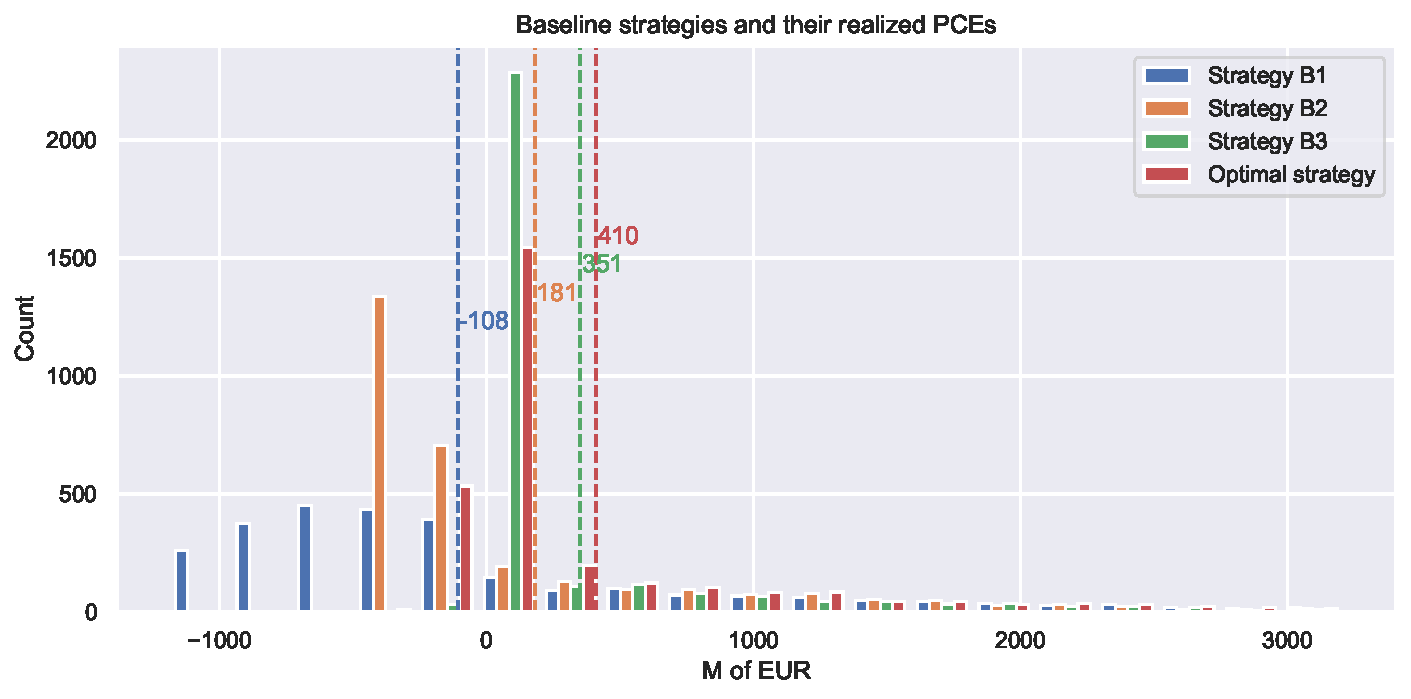
\includegraphics[scale = 0.65]{Images/MT_results_2.pdf}
 		\caption{Comparison of average PCE equivalents of individual strategies, increased volatility.} 
 		\label{fig:Results_increased}
 	\end{center}
 \end{figure}
 

\begin{table}
	\begin{center}
		\begin{tabular}{|l |r |r |r |r|} 
			\hline
			Setup\ Strategy &	Baseline 1 & Baseline 2 & Baseline 3 & Optimal strategy  \\  
			\hline
			Initial setup & -103M & 195M & 330M & 388M \\ 
			\hline
			Increased volatility  & -108M & 181M & 351M & 410M \\
			\hline
		\end{tabular}
	\caption{Comparison of PCE for different strategies and settings.}
	\label{Tab:Result_comparison}
	\end{center}
\end{table}

 
 
 
 

\chapter{Discussion}
We believe that in the presented experiments, we have shown the usage of the SDT-based valuation technique algorithm on an example with a reasonable complexity. We managed to cope with the uncountable state space caused by the assumption of continuous prices and also with the modeling of approximate value functions guided by the theory of ADP. 

The business-specific concepts that we wanted to preserve from the field of capital investment bring after the experiment mixed feelings. The notion of PCE and its usage in the experiment seems to make logical sense. However, the notion of utility and risk-aversion of investors might make better sense in the evaluation of the project as a whole. The usage of utility will be discussed in more detail below. 

\section{Value Function Approximation}
In the first attempts to construct the experiment for this thesis, we came up with a much more complex example than the one finally presented. There were nine elementary states concerning, for example, the government's support of renewable sources of energy, which influenced the future volatility of the power prices. We also firstly introduced actions like mothballing or selling the plant for salvage value. From the study of value function approximations, it seemed like that it will be enough to use only the linear model and choose good basis functions. Nevertheless, we were wrong. 

The complexity and non-linearity of the value functions can be seen in the final simplified example as well. It is clear now that the option-like pattern appears, but the future users of this algorithm need to keep in mind is that the complexity of the project model will most likely be reflected in the complexity of the value functions. 

In our case, three piecewise linear models were enough to cover the state space reasonably, but for more complex models, there might not be such clear patterns as we observed in our example. 

The final choice of a simpler model was motivated by a concern that a more complex value function could take too much of the reader's attention from the main message, which is the illustration of the valuation algorithm itself.

We would like to raise a concern about the possible future adoption of the algorithm from the capital investment companies due to the complexity of the value function modeling for more real-life complex investments. 

\section{Usage of Utility} 
In this thesis, we wanted to preserve the notion of risk-averse investors. We did this by making the optimal decision strategy the one that maximizes the expected utility of the decision-maker (manager of the project) in each decision made. However, when we thought deeper about the global view of investors, the real decision-makers, the incorporation of the risk-aversion through the utility function might have been done differently. 

We have used the utility function for decisions on the micro-level when the project is being further managed. However, in reality, the group of people that make the investment decision does not usually further manage the project. 

On the macro level, the final valuation of a project is usually used for comparison to other investment opportunities, and we believe that this is where the utility function should come into the picture. 

When looking at the results of our simulation, we, for example, see that the baseline strategy B3 is more conservative than the optimal one we derived from our algorithm. Here, we can easily imagine a very risk-averse investor who would prefer the results of strategy B3 over the optimal strategy we have derived. 

Thus, we believe there might be two utility adjustments, first on the micro-level, where the plant manager optimizes the utility of each action. The second utility adjustment for the valuation is for the macro level, where the board of decision-makers will compare individual projects.

\section{Computational Complexity}
In section \ref{Sec:DP} we have talked about the computational complexity of dynamic programming. For our setup of the experiment (with uncountable state space), the DP approach is not even theoretically possible, but we would still like to address the computational complexity and the challenges our algorithm faces. 

We needed to compute three models for each of 300 time epochs. For each model, we needed to have 100 state samples to cover the state space reasonably. For each state, we needed to numerically compute the expected utility, which was in the form of integral, to which we have also used 100 integral samples. This resulted in 90 000 state-utility pairs and 9M of integral samples created as an evolution of state with a length of 5. The computations took several hours on a 2-core device with 16GM of RAM, where it needs to be said that the code was optimized without special care. 

This is to say that more complex valuation problems might also bring with them the need for either faster hardware or better techniques in numerical approximation of integrals and/or more robust models for the value function approximation. 



\section{Experimental Results}
Even though the main focus of the experiments was to present a reasonable illustration of the valuation algorithm we can also see the individual ROA narratives in the results. 

First is the notion that the value of a project increases with the inner uncertainty of its parameters. The value of a project rises together with the volatility from 388M to 410M EUR in our experiment. 

By observing the shapes of histograms of different strategies, we can also observe the narrative of ROA that ``options have value``. The baseline strategy B1 factually represents no options in the ROA sense. We simply build the plant and run it until the end of the observation period. 

The baseline strategy B2 represents the option not to run the plant when the market prices are not favorable. We can see that this option has a significant value, bringing the value of a given project from negative to positive. 

The baseline strategy B3 represents the combination of the time option (waiting for favorable commodity prices) and the option from strategy B2. We see that for our initial state, this option also brings significant value to the project. 

The final remark to the experimental results is that our intuition says that the baseline strategy B3 could be a very good approximation for the optimal strategy derived by our algorithm with a better threshold than 40 EUR. The idea is that for our simple experiment, the optimal strategy simply finds the best thresholds of the spark price to build the first and second block. However, in comparison to B3, the optimal strategy presumably also considers the number of epochs left until the 300 threshold. 


\chapter{Conclusion}
The core message of this thesis is to interpret the problem of project valuation in the form of statistical decision theory. We can declare that the aforementioned contributions of the developed algorithm have been presented by our experiment, most notably in contrast to the current valuation techniques as:

\begin{itemize}
	\item the seamless integration of multiple uncertainty sources;
	\item the integration of continuous probability distribution models of variables; 
	\item the easy representation of actions; 
	\item the increased speed of computation by the usage of ADP algorithm to compute the value function approximations;
	\item the preservation of the domain-specific concepts like the time-value of money and the risk-aversion of investors. 
\end{itemize}

Furthermore, through the thesis, we have discussed other relevant ideas about capital investment, where we believe we can add some value. We talk about the term of utility in a field, which is influenced by it but is not using this notion. We also present the notion of present cash equivalent (PCE), where we argue that for each FCF vector, there is an amount of present cash that the decision-maker is logically indifferent to having now instead of the proposed FCF vector. 


We have demonstrated the discussed ideas and the valuation algorithm on an example of gas power plant valuation. The additional value of the experiment is in the confirmation of the ROA narratives, such as that options have value and that this value rises with the inner uncertainty of the project. 

We have also outlined the limitations of our approach when applied on more complex projects such as: 
\begin{itemize}
	\item complexity of value function models;
	\item numerical integration of continuous state evolutions;
	\item computational complexity driven by both points above.
\end{itemize}

Finally, through the time of writing this thesis, we have identified the following directions for further research: 

\begin{itemize}
	\item valuation of a more complex project in cooperation with an actual investment company;
	\item sensitivity analysis of the time granularity of decisions in our example;
	\item a proper sensitivity analysis of price volatilities in our example;
	\item so-called option games, which combine elements of SDT and game-theory (studying, for example, the optimality of companies' competition vs. collaboration);
	\item model of investments with more complex internal processes than the simple flow process;
	\item a deeper study of the macro vs. micro-optimization of the utility and its effects on consistency of decision making at individual levels of the investment. 
\end{itemize}


\pagestyle{plain}
\bibliographystyle{plain}
\bibliography{fr}

\end{document}
